\chapter{Dynamic Programming}
\section{Thinking in Dynamic Programming}
{\color{blue}{Dynamic programming}}, like {\color{blue}{recursion}}, solves a problem by tackling {\color{blue}{smaller versions of the same problem}} and then combining those solutions to solve the original problem. However, dynamic programming {\color{blue}{solves each subproblem only once}} and stores its result somewhere, thereby avoiding the redundant work of recomputing solutions to subproblems. \\

Dynamic programming is typically applied to {\color{blue}{optimization problems}}. Such problems can have many possible solutions. Each solution has a value, and we wish to find a solution with the {\color{blue}{optimal value}}. We call such a solution {\color{blue}{an optimal solution}} to the problem, as opposed to {\color{blue}{the optimal solution}}, since there may be several solutions that achieve the optimal value.\\

Key characteristics indicating a problem is suitable for dynamic programming include:
\begin{itemize}
	\item {\color{blue}{[Optimal substructure]}} A problem is said to have an optimal substructure if an optimal solution to the problem contains optimal solutions to its subproblems. This means that the problem can be broken down into smaller, more manageable parts, and solving these smaller parts optimally helps in finding the optimal solution to the larger problem.
	\item {\color{blue}{[Overlapping subproblems]}} This refers to the scenario where the problem can be broken down into subproblems, but these subproblems are not independent; they overlap. In other words, the same subproblems are solved multiple times. Dynamic programming takes advantage of this by solving each subproblem only once and storing its solution, thus avoiding the computation of the same problem again.
\end{itemize}

\subsection{Steps to Solve DP Problems}
The general steps to solve a problem by dynamic programming are as follows.

\begin{enumerate}
\item Define the smaller {\color{blue}{subproblems}} that make up the original problem.
\item Utilize {\color{blue}{solutions to the smaller subproblems}} to construct the {\color{blue}{solution the solution to the original problem}}. This is typically done in a bottom-up fashion.
\end{enumerate}

Note that:
\begin{itemize}
\item Since some solutions depend on others, you should be careful about {\color{blue}{the order in which you solve the subproblems}}.
\item Distinguish between finding the {\color{blue}{optimal value}} (the best numerical answer) and the {\color{blue}{optimal solution}} (the decisions or path that leads to this best value). If you need to reconstruct the optimal solution, you may need to implement additional structures or mechanisms to track the decisions leading to the optimal values.
\end{itemize}

\subsection{Steps to Solve DP Problems on LeetCode}
For DP problems on LeetCode, the practical steps are as follows.
\begin{enumerate}
\item Define the {\color{blue}{DP table}}, ensuring you fully understand the meanings of its {\color{blue}{elements}} and {\color{blue}{subscripts}}.
\item Determine the {\color{blue}{transition function}}
\item {\color{blue}{Initialize}} the DP table with the {\color{blue}{base cases}}.
\item Determine the {\color{blue}{order}} to fill out the DP table.
\end{enumerate}

The first two steps determine the general logic of the solution, and the last two steps are about the implementation details.\\

In addition, if your code doesn't output the correct result, print out each element of the DP array in algorithm's execution order and check what went wrong.

%\subsection{Map Between Entries of DP Vector and Specific Scenarios}
%Pay attention to how we link each entry in the DP vector to specific scenarios.
%
%\subsubsection*{Position-Based Problems}
%When the problem is {\color{blue}{position-based}}, each entry in the DP table corresponds to a specific {\color{blue}{position}} in the problem.\\
%
%By default, a DP vector is {\colorbox{CodeBackground}{\lstinline|0|}}-indexed:
%\begin{itemize}
%\item For a {\colorbox{CodeBackground}{\lstinline|0|}}-indexed scenario, {\colorbox{CodeBackground}{\lstinline|dp[i]|}} corresponds to the {\colorbox{CodeBackground}{\lstinline|i|}}th position of the problem.
%\item For a {\colorbox{CodeBackground}{\lstinline|1|}}-indexed scenario, {\colorbox{CodeBackground}{\lstinline|dp[i]|}} corresponds to the {\colorbox{CodeBackground}{\lstinline|(i+1)|}}th position of the problem.
%\end{itemize}
%
%\subsubsection*{Amount/Length-Based Problems}
%When the problem is {\color{blue}{amount/length-based}}, each entry in the DP table corresponds to a specific amount/length in the problem. Thus:
%\begin{itemize}
%\item {\colorbox{CodeBackground}{\lstinline|dp[0]|}} corresponds to the {\color{blue}{empty case}}.
%\item For {\colorbox{CodeBackground}{\lstinline|i > 0|}}, {\colorbox{CodeBackground}{\lstinline|dp[i]|}} corresponds to {\color{blue}{amount/length}} {\colorbox{CodeBackground}{\lstinline|i|}}.
%\end{itemize}

\subsection{Relationship between DP and Recursion}
{\color{ForestGreen}{DP = Recursion + Memorization}}\\

Both {\color{blue}{dynamic programming}} and {\color{blue}{recursion}} solve a problem by tackling {\color{blue}{smaller versions of the same problem}} and then combining those solutions to solve the original problem. Consequently, you might see some problems can be solved by both methods. However, dynamic programming solves each subproblem only once and stores its result somewhere ({\color{blue}{memorization}}), thereby avoiding the redundant work of recomputing solutions to subproblems.

\subsection{Relationship between DP and Greedy Algorithms}\label{subsec:relationship_between_dp_greedy}
Both {\color{blue}{dynamic programming}} and {\color{blue}{greedy algorithms}} are typically applied to {\color{blue}{optimization problems}}. So, you might see many problems can be solved by both methods. \\

{\color{blue}{Dynamic programming}} and {\color{blue}{greedy algorithms}} solve problems in distinct ways.
\begin{itemize}
	\item {\color{blue}{Dynamic programming}} breaks down a problem into {\color{blue}{smaller versions of the same problem}}. It then combines the solutions of these {\color{blue}{subproblems}} to formulate the final solution.
	\item {\color{blue}{Greedy algorithms}} break down a problem into {\color{blue}{a sequence of consistent steps}}. At each step, it chooses the {\color{blue}{greedy choice}} to reach the {\color{blue}{local optimum}}. Through this heuristic process, it often succeeds in approximating the {\color{blue}{global optimum}}.
\end{itemize}

In addition, {\color{blue}{dynamic programming}} guarantees the {\color{blue}{global optimum}} and {\color{blue}{greedy algorithms}} don't. 

\section{Thinking in Knapsack Problem}
\subsection{0/1 Knapsack Problem}
\subsubsection{Problem Formulation}
There is {\color{blue}{a knapsack}} with capacity {\color{blue}{$W$}}. \\

There are {\color{blue}{$n$ items}}, whose {\color{blue}{weights}} are {\color{blue}{$\left[w_0, w_1, \ldots, w_{n-1}\right]$}} and the corresponding \ul{non-negative} {\color{blue}{values}} are {\color{blue}{$\left[v_0, v_2, \ldots, v_{n-1}\right]$}}. \\

Our goal is to select some items to be put into the knapsack such that {\color{blue}{the total value of those items is maximized}}. That is, the sum of the weight of those selected items cannot exceed $W$, and we want the total value of those items to be as large as possible.\\

It should be noted that, {\color{blue}{in the 0/1 knapsack problem, each item can only be used once.}}

\subsubsection{Analysis - $2$D DP Table}
We define {\color{blue}{$ dp[i, j] $}} to be the maximum possible value of a knapsack with {\color{blue}{capacity $ j $}} and can use the {\color{blue}{first $ i $ items}}. \\

The answer to the original problem is {\color{blue}{$ dp[n, W] $}}.\\

{\color{ForestGreen}{For each item $i$, we can choose to either put it into the knapsack or not}}, so the transition function is defined as follows.
\begin{equation}
{\color{blue}{
dp[i, j] = 
\begin{cases} 
    dp[i - 1, j] & \text{if}\ j < w_{i-1}\\
    \max\left\{dp[i - 1, j], dp[i - 1, j - w_{i-1}] + v_{i-1}\right\} & \text{if}\ j \geq w_{i-1}
\end{cases}
}}
\end{equation}

The pesudocode for 0/1 knapsack problem is listed as follows.
\begin{algorithm}[H]\label{algorithm:01_knapsack_problem_1}
\caption{DP Algorithm for 0/1 Knapsack Problem}
\begin{algorithmic}[1]
\For{$i = 0$ to $n$} \Comment{base cases: no capacity}
    \State $dp[i, 0] = 0$;
\EndFor
\For{$j = 0$ to $W$}  \Comment{base cases: no items}
    \State $dp[0, j] = 0$;
\EndFor
\For{$i = 1$ to $n$}
    \For{$j = 1$ to $W$}
        \State 
        $dp[i, j] = 
        \begin{cases} 
            dp[i - 1, j] & \text{if}\ j < w_{i-1}\\
            \max\left\{dp[i - 1, j], dp[i - 1, j - w_{i-1}] + v_{i-1}\right\} & \text{if}\ j \geq w_{i-1}
        \end{cases}$
    \EndFor
\EndFor
\State \textbf{return} $dp[n, W]$;
\end{algorithmic}
\end{algorithm}

Let's consider an example of 0/1 knapsack problem:
\begin{itemize}
\item There are $5$ items, with $\text{weights} = \left[1, 2, 3, 6, 12\right]$ and $\text{values} =  \left[2, 1, 4, 7, 10\right]$.
\item The capacity of the knapsack is $W = 10$.
\end{itemize}

The C++ code is as follows.
\begin{lstlisting}
int Knapsack2D(const std::vector<int>& weights, const std::vector<int>& values,
               int capacity) {
  // dp[i][j] - maximum value of the first i items with a capacity of j
  std::vector<std::vector<int>> dp(weights.size() + 1, std::vector<int>(capacity + 1, 0));
  for (int i = 1; i <= weights.size(); ++i) {
    for (int j = 1; j <= capacity; ++j) {
      if (j < weights[i - 1]) {
        dp[i][j] = dp[i - 1][j];
      } else {
        dp[i][j] = std::max(dp[i - 1][j], dp[i - 1][j - weights[i - 1]] + values[i - 1]);
      }
    }
  }
  return dp[weights.size()][capacity];
}
\end{lstlisting}

The DP Table is as follows.
\begin{table}[H]
\centering
\begin{tabular}{cc|c|c|c|c|c|c|c|c|c|c|c|c|}
\hline
weight & value & i/j & 0 & 1 & 2 & 3 & 4 & 5 & 6 & 7 & 8 & 9 & 10 \\ \hline
- & - & 0   & 0 & 0 & 0 & 0 & 0 & 0 & 0 & 0 & 0 & 0 & 0  \\ \hline
1 & 2 & 1   & 0 & 2 & 2 & 2 & 2 & 2 & 2 & 2 & 2 & 2 & 2  \\ \hline
2 & 1 & 2   & 0 & 2 & 2 & 3 & 3 & 3 & 3 & 3 & 3 & 3 & 3  \\ \hline
3 & 4 & 3   & 0 & 2 & 2 & 4 & 6 & 6 & 7 & 7 & 7 & 7 & 7  \\ \hline
6 & 7 & 4   & 0 & 2 & 2 & 4 & 6 & 6 & 7 & 9 & 9 & 11 & 13 \\ \hline
12 & 10 & 5   & 0 & 2 & 2 & 4 & 6 & 6 & 7 & 9 & 9 & 11 & 13 \\ \hline
\end{tabular}
\caption{DP Table for 0/1 Knapsack Problem}
\end{table}

Because {\color{blue}{$dp[i][j]$ depends only on the entries to its left in the previous row ($i-1$) and the entry directly above it}}, you can change the order to fill out the DP table as long as you respect this dependency.\\

For example, you could swap the order of the outer loop for $i$ with the inner loop for $j$.
\begin{algorithm}[H]\label{algorithm:01_knapsack_problem_2}
\caption{DP Algorithm for 0/1 Knapsack Problem}
\begin{algorithmic}[1]
\For{$i = 0$ to $n$} \Comment{base cases: no capacity}
    \State $dp[i, 0] = 0$;
\EndFor
\For{$j = 0$ to $W$}  \Comment{base cases: no items}
    \State $dp[0, j] = 0$;
\EndFor
\For{{\color{magenta}{$j = 1$ to $W$}}}
    \For{{\color{magenta}{$i = 1$ to $n$}}}
        \State 
        $dp[i, j] = 
        \begin{cases} 
            dp[i - 1, j] & \text{if}\ j < w_{i-1}\\
            \max\left\{dp[i - 1, j], dp[i - 1, j - w_{i-1}] + v_{i-1}\right\} & \text{if}\ j \geq w_{i-1}
        \end{cases}$
    \EndFor
\EndFor
\State \textbf{return} $dp[n, W]$;
\end{algorithmic}
\end{algorithm}

The C++ code is as follows and the DP table is the same.
\begin{lstlisting}
int Knapsack2D(const std::vector<int>& weights, const std::vector<int>& values,
                 int capacity) {
  std::vector<std::vector<int>> dp(weights.size() + 1, std::vector<int>(capacity + 1, 0));
  for (int j = 1; j <= capacity; ++j) {
    for (int i = 1; i <= weights.size(); ++i) {
      if (j < weights[i - 1]) {
        dp[i][j] = dp[i - 1][j];
      } else {
        dp[i][j] = std::max(dp[i - 1][j], dp[i - 1][j - weights[i - 1]] + values[i - 1]);
      }
    }
  }
  return dp[weights.size()][capacity];
}
\end{lstlisting}

For another example, you could also reverse the loop for $j$.
\begin{algorithm}[H]\label{algorithm:01_knapsack_problem_3}
\caption{DP Algorithm for 0/1 Knapsack Problem}
\begin{algorithmic}[1]
\For{$i = 0$ to $n$} \Comment{base cases: no capacity}
    \State $dp[i, 0] = 0$;
\EndFor
\For{$j = 1$ to $W$}  \Comment{base cases: no items}
    \State $dp[0, j] = 0$;
\EndFor
\For{$i = 1$ to $n$}
    \For{{\color{magenta}{$j = W$ to $1$}}}
        \State 
        $dp[i, j] = 
        \begin{cases} 
            dp[i - 1, j] & \text{if}\ j < w_{i-1}\\
            \max\left\{dp[i - 1, j], dp[i - 1, j - w_{i-1}] + v_{i-1}\right\} & \text{if}\ j \geq w_{i-1}
        \end{cases}$
    \EndFor
\EndFor
\State \textbf{return} $dp[n, W]$;
\end{algorithmic}
\end{algorithm}
The C++ code is as follows and the DP table is the same.
\begin{lstlisting}
int Knapsack2D(const std::vector<int>& weights, const std::vector<int>& values,
               int capacity) {
  std::vector<std::vector<int>> dp(weights.size() + 1, std::vector<int>(capacity + 1, 0));
  for (int i = 1; i <= weights.size(); ++i) {
    for (int j = capacity; j >= 1; --j) {
      if (j < weights[i - 1]) {
        dp[i][j] = dp[i - 1][j];
      } else {
        dp[i][j] = std::max(dp[i - 1][j], dp[i - 1][j - weights[i - 1]] + values[i - 1]);
      }
    }
  }
  return dp[weights.size()][capacity];
}
\end{lstlisting}

\subsubsection{Analysis - $1$D DP Vector}
The 1D solution saves space by cleverly overwritten entries in the 2D DP table that are no longer needed. It is really important to realize that this solution is a simulation of the 2D solution. That is to say, if your code isn't working as expected, you should start debugging with the 2D solution and then convert it into the 1D solution.\\

We define {\color{blue}{$ dp[j] $}} to be the maximum possible value of a knapsack with {\color{blue}{capacity $ j $}} and can use all items.\\

The answer to the original problem is {\color{blue}{$ dp[W] $}}.\\

{\color{ForestGreen}{For each item $i$, we can choose to either put it into the knapsack or not}}, so the transition function is defined as follows.
\begin{equation}
{\color{blue}{
dp[j] = 
\begin{cases} 
    dp[j] & \text{if}\ j < w_{i-1}\\
    \max\left\{dp[j], dp[j - w_{i-1}] + v_{i-1}\right\} & \text{if}\ j \geq w_{i-1} 
\end{cases}
}}
\end{equation}

The pesudocode for the 0/1 knapsack problem is listed as follows.
\begin{algorithm}[H]
\caption{DP Algorithm for 0/1 Knapsack Problem}
\begin{algorithmic}[1]
\State $dp[0] = 0$ \Comment{base case: no capacity}
\For{{\color{blue}{$i = 1$ to $n$}}}
    \For{{\color{blue}{$j = W$ to $w_{i-1}$}}}
        \State  $dp[j] = \max\left\{dp[j], dp[j - w_{i-1}] + v_{i-1}\right\}$\Comment{handle the case of $j < w_{i-1}$ by not overwriting it}
    \EndFor
\EndFor
\State \textbf{return} $dp[W]$;
\end{algorithmic}
\end{algorithm}

Be careful of the order to fill out the DP table, that's the only way we can simulate the 2D solution.
\begin{itemize}
\item Swapping the order of the outer loop for $i$ with the inner loop for $j$ is not feasible. Doing so would mean when we try to calculate $dp[i][j]$, we wouldn't be able to find the correct to its left in the previous row ($i-1$) because it has been overwritten.
\item Iterating $j$ from $1$ to $W$ is not feasible. Doing so would mean when we try to calculate $dp[i][j]$, we wouldn't be able to find the correct to its left in the previous row ($i-1$) because it has been overwritten.
\end{itemize}

The C++ code is as follows.
\begin{lstlisting}
int Knapsack1D(const std::vector<int>& weights, const std::vector<int>& values,
               int capacity) {
  std::vector<int> dp(capacity + 1, 0);
  for (int i = 1; i <= weights.size(); ++i) {
    for (int j = capacity; j >= weights[i - 1]; --j) {
      dp[j] = std::max(dp[j], dp[j - weights[i - 1]] + values[i - 1]);
    }
  }
  return dp[capacity];
}
\end{lstlisting}

The DP vector is as follows.
\begin{table}[H]
\centering
\begin{tabular}{|c|c|c|c|c|c|c|c|c|c|c|}
\hline
0 & 2 & 2 & 4 & 6 & 6 & 7 & 9 & 9 & 11 & 13 \\
\hline
\end{tabular}
\caption{DP Vector for 0/1 Knapsack Problem}
\end{table}

\subsubsection{Generalization of 0/1 Knapsack Problem}
In the analysis above, we highlight the expression:
\begin{center}
{\color{ForestGreen}{For each item $i$, we can choose to either put it into the knapsack or not}}, ...
\end{center}
It means that $dp[i][j]$ can be derived from {\color{blue}{$dp[i-1][j]$ (doesn't put item $i$ into the knapsack)}} and {\color{blue}{$dp[i][j-w_{i-1}]$ (put the item $i$ into the knapsack)}}, which is the key characteristic of the 0/1 knapsack problem. While the classic 0/1 knapsack problem focuses on maximizing value, we can adapt this objective to others, like minimizing value, without changing the basic approach.  So, once a problem has such feature, try to use a 2D DP Table to solve it and then convert it into the 1D DP Vector solution. \\

See \hyperref[subsubsec:01_knapsack_oj_problems]{Related OJ Problems} for more examples.

\subsubsection{Related OJ Problems}\label{subsubsec:01_knapsack_oj_problems}
\begin{itemize}
\item \hyperref[lc0416]{LC 0416 - Partition Equal Subset Sum}
\item \hyperref[lc1049]{LC 1049 - Last Stone Weight II}
\item \hyperref[lc0494]{LC 0494 - Target Sum}
\item \hyperref[lc0474]{LC 0474 - Ones and Zeroes}
\end{itemize}

\subsection{Unbounded Knapsack Problem}
\subsubsection{Problem Formulation}
There is {\color{blue}{a knapsack}} with capacity {\color{blue}{$W$}}. \\

There are {\color{blue}{$n$ types of items}}, whose {\color{blue}{weights}} are {\color{blue}{$\left[w_0, w_1, \ldots, w_{n-1}\right]$}} and the corresponding \ul{non-negative} {\color{blue}{values}} are {\color{blue}{$\left[v_0, v_2, \ldots, v_{n-1}\right]$}}. \\

Our goal is to select some items to be put into the knapsack such that {\color{blue}{the total value of those items is maximized}}. That is, the sum of the weight of those selected items cannot exceed $W$, and we want the total value of those items to be as large as possible.\\

It should be noted that, {\color{blue}{in the unbounded knapsack problem, you can use each type of item as many times as needed.}}

\subsubsection{Analysis - $2$D DP Table}
We define {\color{blue}{$ dp[i, j] $}} to be the maximum possible value of a knapsack with {\color{blue}{capacity $ j $}} and can use the {\color{blue}{first $ i $ types of items}}. \\

The answer to the original problem is {\color{blue}{$ dp[n, W] $}}.\\

{\color{ForestGreen}{For each item $i$, we can choose to either put it into the knapsack or not}}, so the transition function is defined as follows.
\begin{equation}
{\color{blue}{
dp[i, j] = 
\begin{cases} 
    dp[i - 1, j] & \text{if}\ j < w_{i-1}\\
    \max\left\{dp[i - 1, j], dp[i, j - w_{i-1}] + v_{i-1}\right\} & \text{if}\ j \geq w_{i-1}
\end{cases}
}}
\end{equation}

The pesudocode for the unbounded knapsack problem is listed as follows.
\begin{algorithm}[H]\label{algorithm:unbounded_knapsack_problem_1}
\caption{DP Algorithm for Unbounded Knapsack Problem}
\begin{algorithmic}[1]
\For{$i = 0$ to $n$} \Comment{base cases: no capacity}
    \State $dp[i, 0] = 0$;
\EndFor
\For{$j = 0$ to $W$}  \Comment{base cases: no items}
    \State $dp[0, j] = 0$;
\EndFor
\For{$i = 1$ to $n$}
    \For{$j = 1$ to $W$}
        \State 
        $dp[i, j] = 
        \begin{cases} 
            dp[i - 1, j] & \text{if}\ j < w_{i-1}\\
            \max\left\{dp[i - 1, j], dp[i, j - w_{i-1}] + v_{i-1}\right\} & \text{if}\ j \geq w_{i-1}
        \end{cases}$
    \EndFor
\EndFor
\State \textbf{return} $dp[n, W]$;
\end{algorithmic}
\end{algorithm}

Let's consider an example of unbounded knapsack problem:
\begin{itemize}
\item There are $5$ items, with $\text{weights} = \left[1, 2, 4, 5, 6\right]$ and $\text{values} =  \left[1, 3, 5, 6, 10\right]$.
\item The capacity of the knapsack is $W = 10$.
\end{itemize}

The C++ code is as follows.
\begin{lstlisting}
int Knapsack2D(const std::vector<int>& weights, const std::vector<int>& values,
               int capacity) {
  std::vector<std::vector<int>> dp(weights.size() + 1, std::vector<int>(capacity + 1, 0));
  for (int i = 1; i <= weights.size(); ++i) {
    for (int j = 1; j <= capacity; ++j) {
      if (j < weights[i - 1]) {
        dp[i][j] = dp[i - 1][j];
      } else {
        dp[i][j] = std::max(dp[i - 1][j], dp[i][j - weights[i - 1]] + values[i - 1]);
      }
    }
  }
  return dp[weights.size()][capacity];
}
\end{lstlisting}

The DP table is as follows.

\begin{table}[H]
\centering
\begin{tabular}{cc|c|c|c|c|c|c|c|c|c|c|c|c|}
\hline
weight & value & i/j & 0 & 1 & 2 & 3 & 4 & 5 & 6 & 7 & 8 & 9 & 10 \\ \hline
- & - & 0   & 0 & 0 & 0 & 0 & 0 & 0 & 0 & 0 & 0 & 0 & 0  \\ \hline
1 & 1 & 1   & 0 & 1 & 2 & 3 & 4 & 5 & 6 & 7 & 8 & 9 & 10 \\ \hline
2 & 3 & 2   & 0 & 1 & 3 & 4 & 6 & 7 & 9 & 10 & 12 & 13 & 15 \\ \hline
4 & 5 & 3   & 0 & 1 & 3 & 4 & 6 & 7 & 9 & 10 & 12 & 13 & 15 \\ \hline
5 & 6 & 4   & 0 & 1 & 3 & 4 & 6 & 7 & 9 & 10 & 12 & 13 & 15 \\ \hline
6 & 10 & 5   & 0 & 1 & 3 & 4 & 6 & 7 & 10 & 11 & 13 & 14 & 16 \\ \hline
\end{tabular}
\caption{DP Table for Unbounded Knapsack Problem}
\label{tab:unbounded_knapsack_dp}
\end{table}

In this case, {\color{blue}{$dp[i][j]$ depends only on the entries to its left in the same row ($i$), and the entry directly above it}}, you can change the order to fill out the DP table as long as you respect this dependency.\\

For example, you can swap the order of the outer loop for $i$ with the inner loop for $j$.
\begin{algorithm}[H]\label{algorithm:unbounded_knapsack_problem_2}
\caption{DP Algorithm for Unbounded Knapsack Problem}
\begin{algorithmic}[1]
\For{$i = 0$ to $n$} \Comment{base cases: no capacity}
    \State $dp[i, 0] = 0$;
\EndFor
\For{$j = 0$ to $W$}  \Comment{base cases: no items}
    \State $dp[0, j] = 0$;
\EndFor
\For{{\color{magenta}{$j = 1$ to $W$}}}
    \For{{\color{magenta}{$i = 1$ to $n$}}}
        \State 
        $dp[i, j] = 
        \begin{cases} 
            dp[i - 1, j] & \text{if}\ j < w_{i-1}\\
            \max\left\{dp[i - 1, j], dp[i, j - w_{i-1}] + v_{i-1}\right\} & \text{if}\ j \geq w_{i-1}
        \end{cases}$
    \EndFor
\EndFor
\State \textbf{return} $dp[n, W]$;
\end{algorithmic}
\end{algorithm}

The C++ code is as follows and the DP table is the same.
\begin{lstlisting}
int Knapsack2D(const std::vector<int>& weights, const std::vector<int>& values,
               int capacity) {
  std::vector<std::vector<int>> dp(weights.size() + 1, std::vector<int>(capacity + 1, 0));
  for (int j = 1; j <= capacity; ++j) {
    for (int i = 1; i <= weights.size(); ++i) {
      if (j < weights[i - 1]) {
        dp[i][j] = dp[i - 1][j];
      } else {
        dp[i][j] = std::max(dp[i - 1][j], dp[i][j - weights[i - 1]] + values[i - 1]);
      }
    }
  }
  return dp[weights.size()][capacity];
}
\end{lstlisting}

However, reversing the loop for $j$ gives us the wrong solution. Doing so would mean when we try to calculate $dp[i][j]$, we wouldn't be able to find the correct entry to its left in the same row ($i$).

\subsubsection{Analysis - $1$D DP Vector}
The 1D solution saves space by cleverly overwritten entries in the 2D DP table that are no longer needed. It is really important to realize that this solution is a simulation of the 2D solution. That is to say, if your code isn't working as expected, you should start debugging with the 2D solution and then convert it into the 1D solution.\\

We define {\color{blue}{$ dp[j] $}} to be the maximum possible value of a knapsack with {\color{blue}{capacity $ j $}} and can use all items.\\

The answer to the original problem is {\color{blue}{$ dp[W] $}}.\\

{\color{ForestGreen}{For each item $i$, we can choose to either put it into the knapsack or not}}, so the transition function is defined as follows.
\begin{equation}
{\color{blue}{
dp[j] = 
\begin{cases} 
    dp[j] & \text{if}\ j < w_{i-1}\\
    \max\left\{dp[j], dp[j - w_{i-1}] + v_{i-1}\right\} & \text{if}\ j \geq w_{i-1} 
\end{cases}
}}
\end{equation}

The pesudocode for the unbounded knapsack kroblem is listed as follows.
\begin{algorithm}[H]
\caption{DP Algorithm for Unbounded Knapsack Problem}
\begin{algorithmic}[1]
\State $dp[0] = 0$ \Comment{base case: no capacity}
\For{{\color{blue}{$i = 1$ to $n$}}}
    \For{{\color{blue}{$j = 1$ to $W$}}}
        \State $dp[j] = \max\left\{dp[j], dp[j - w_{i-1}] + v_{i-1}\right\} $ \Comment{handle the case of $j < w_{i-1}$ by not overwriting it}
    \EndFor
\EndFor
\State \textbf{return} $dp[W]$;
\end{algorithmic}
\end{algorithm}

The C++ code is as follows.
\begin{lstlisting}
int Knapsack1D(const std::vector<int>& weights, const std::vector<int>& values,
               int capacity) {
  std::vector<int> dp(capacity + 1, 0);
  for (int i = 1; i <= weights.size(); ++i) {
    for (int j = 1; j <= capacity; ++j) {
      if (j >= weights[i - 1]) {
        dp[j] = std::max(dp[j], dp[j - weights[i - 1]] + values[i - 1]);
      }
    }
  }
  return dp[capacity];
}
\end{lstlisting}

The DP vector is as follows.
\begin{table}[H]
\centering
\begin{tabular}{|c|c|c|c|c|c|c|c|c|c|c|}
\hline
0 & 2 & 2 & 4 & 6 & 6 & 7 & 9 & 9 & 11 & 13 \\
\hline
\end{tabular}
\caption{DP Vector for Unbounded Knapsack Problem}
\end{table}

We can also change the order of the outer loop for $i$ and the inner loop for $j$ to simulate the 2D solution.

\begin{algorithm}[H]
\caption{DP Algorithm for Unbounded Knapsack Problem}
\begin{algorithmic}[1]
\State $dp[0] = 0$ \Comment{base case: no capacity}
\For{{\color{blue}{$j = 1$ to $W$}}}
    \For{{\color{blue}{$i = 1$ to $n$}}}
        \State 
        $dp[j] = 
        \begin{cases} 
            dp[j] & \text{if}\ j < w_{i-1}\\
            \max\left\{dp[j], dp[j - w_{i-1}] + v_{i-1}\right\} & \text{if}\ j \geq w_{i-1} 
        \end{cases}$\Comment{handle the case of $j < w_{i-1}$ by not overwriting it}
    \EndFor
\EndFor
\State \textbf{return} $dp[W]$;
\end{algorithmic}
\end{algorithm}

The C++ code is as follows and the DP vector is the same.
\begin{lstlisting}
int Knapsack1D(const std::vector<int>& weights, const std::vector<int>& values,
                 int capacity) {
  std::vector<int> dp(capacity + 1, 0);
  for (int j = 1; j <= capacity; ++j) {
    for (int i = 1; i <= weights.size(); ++i) {
      if (j >= weights[i - 1]) {
        dp[j] = std::max(dp[j], dp[j - weights[i - 1]] + values[i - 1]);
      }
    }
  }
  return dp[capacity];
}
\end{lstlisting}

However, reversing the loop for $j$ gives us the wrong solution. Doing so would mean when we try to calculate $dp[i][j]$, we wouldn't be able to find the correct entry to its left in the same row ($i$).

\subsubsection{Generalization of Unbounded Knapsack Problem}
In the analysis above, we highlight the expression:
\begin{center}
{\color{ForestGreen}{For each item $i$, we can choose to either put it into the knapsack or not}}, ...
\end{center}
It means that $dp[i][j]$ can be derived from {\color{blue}{$dp[i-1][j]$ (doesn't put item $i$ into the knapsack)}} and {\color{blue}{$dp[i][j-w_{i-1}]$ (put the item $i$ into the knapsack)}}, which is the key characteristic of the unbounded knapsack problem. While the classic unbounded knapsack problem focuses on maximizing value, we can adapt this objective to others, like minimizing value, without changing the basic approach. So, once a problem has such feature, try to use a 2D DP Table to solve it and then convert it into the 1D DP Vector solution. \\

See \hyperref[subsubsec:unbounded_knapsack_oj_problems]{Related OJ Problems} for more examples.

\subsubsection{Related OJ Problems}\label{subsubsec:unbounded_knapsack_oj_problems}
\begin{itemize}
\item \hyperref[lc0322]{LC 0322 - Coin Change}
\item \hyperref[lc0518]{LC 0518 - Coin Change II}
\item \hyperref[lc0279]{LC 0279 - Perfect Squares}
\end{itemize}

\subsection{Bounded Knapsack Problem}

\subsection{Multiple Knapsack Problem}

\section{LC 0509 - Fibonacci Sequence}
The following is the \ul{Fibonacci Sequence} starting from {\colorbox{CodeBackground}{\lstinline|0|}} and {\colorbox{CodeBackground}{\lstinline|1|}}:
\begin{itemize}
\item {\colorbox{CodeBackground}{\lstinline|F(0) = 0|}};
\item {\colorbox{CodeBackground}{\lstinline|F(1) = 1|}};
\item {\colorbox{CodeBackground}{\lstinline|F(n) = F(n - 1) + F(n - 2)|}}, for {\colorbox{CodeBackground}{\lstinline|n > 1|}}.
\end{itemize}

Given {\colorbox{CodeBackground}{\lstinline|n|}}, calculate {\colorbox{CodeBackground}{\lstinline|F(n)|}}.

\subsection*{Solution 1 - DP}\label{solution:lc0509_dp}
\begin{lstlisting}
int fib(int n) {
  if (n <= 1) { return n; }
  // dp[i] = fib(i)
  std::vector<int> dp(n + 1, 0);
  dp[0] = 0;
  dp[1] = 1;
  for (int i = 2; i <= n; ++i) { dp[i] = dp[i - 1] + dp[i - 2]; }
  return dp.back();
}
\end{lstlisting}

\subsection*{Solution 2 - DP, Optimized (Fibonacci Sequence)}\label{solution:lc0509_fibonacci_sequence}
\begin{lstlisting}
int fib(int n) {
  if (n <= 1) { return n; }
  int a = 0;
  int b = 1;
  int c = 0;
  for (int i = 2; i <= n; ++i) {
    c = a + b;
    a = b;
    b = c;
  }
  return b;
}
\end{lstlisting}

\subsection*{Other Solutions}
\begin{itemize}
%\item \hyperref[solution:lc0509_dp]{DP}
%\item \hyperref[solution:lc0509_fibonacci_sequence]{DP, Optimized (Fibonacci Sequence)}
\item \hyperref[solution:lc0509_recursion]{Recursion}
\end{itemize}

\section{LC 0070 - Climbing Stairs}
You are climbing a staircase with {\colorbox{CodeBackground}{\lstinline|n|}} steps. Each time you can either climb {\colorbox{CodeBackground}{\lstinline|1|}} or {\colorbox{CodeBackground}{\lstinline|2|}} steps. In how many distinct ways can you climb to the top?

\subsection*{Solution 1 - DP}\label{solution:lc0070_dp}
\begin{lstlisting}
int climbStairs(int n) {
  // edge cases
  if (n <= 2) { return n; }
  // dp[i] = number of ways to climb to (i+1)th stair
  std::vector<int> dp(n, 0);
  dp[0] = 1;
  dp[1] = 2;
  for (int i = 2; i < n; ++i) { dp[i] = dp[i - 1] + dp[i - 2]; }
  return dp.back();
}
\end{lstlisting}

\subsection*{Solution 2 - DP, Optimized (Fibonacci Sequence)}\label{solution:lc0070_fibonacci_sequence}
\begin{lstlisting}
int climbStairs(int n) {
  if (n <= 2) { return n; }
  int a = 1;
  int b = 2;
  int c = 0;
  for (int i = 3; i <= n; ++i) {
    c = a + b;
    a = b;
    b = c;
  }
  return b;
}
\end{lstlisting}

\subsection*{Other Solutions}
\begin{itemize}
%\item \hyperref[solution:lc0070_dp]{DP}
%\item \hyperref[solution:lc0070_fibonacci_sequence]{DP, Optimized (Fibonacci Sequence)}
\item \hyperref[solution:lc0070_recursion]{Recursion}
\end{itemize}

\section{LC 0198 - House Robber}\label{lc0198}
You are a professional robber planning to rob houses along a street. Each house has a certain amount of money stashed, the only constraint stopping you from robbing each of them is that adjacent houses have security systems connected and it will automatically contact the police if two adjacent houses were broken into on the same night.\\

Given a \ul{non-empty} integer array {\colorbox{CodeBackground}{\lstinline|nums|}} representing the amount of money of each house, return the maximum amount of money you can rob tonight without alerting the police.\\

Examples:
\begin{itemize}
\item {\colorbox{CodeBackground}{\lstinline|[1,2,3,1] --> 4 (1 + 3)|}}
\item {\colorbox{CodeBackground}{\lstinline|[2,7,9,3,1] --> 12 (2 + 9 + 1)|}}
\end{itemize}

\subsection*{Solution - DP}
\begin{lstlisting}
int rob(std::vector<int>& nums) {
  // edge case
  if (nums.size() == 1) { return nums[0]; }
  // dp[i] - max amount of money that can be robbed from houses 0 to i
  std::vector<int> dp(nums.size(), 0);
  dp[0] = nums[0];
  dp[1] = std::max(nums[0], nums[1]);
  for (int i = 2; i < nums.size(); ++i) { dp[i] = std::max(dp[i - 2] + nums[i], dp[i - 1]); }
  return dp.back();
}
\end{lstlisting}

\subsection*{Related}
\begin{itemize}
\item \hyperref[lc0198]{LC 0198 - House Robber}
\item \hyperref[lc0213]{LC 0213 - House Robber II}
\item \hyperref[lc0337]{LC 0337 - House Robber III}
\end{itemize}

\section{LC 0213 - House Robber II}\label{lc0213}
You are a professional robber planning to rob houses along a street. Each house has a certain amount of money stashed. All houses at this place are \ul{arranged in a circle}. That means the first house is the neighbor of the last one. Meanwhile, adjacent houses have a security system connected, and it will automatically contact the police if two adjacent houses were broken into on the same night.\\

Given a \ul{non-empty} integer array {\colorbox{CodeBackground}{\lstinline|nums|}} representing the amount of money of each house, return the maximum amount of money you can rob tonight without alerting the police.\\

Examples:
\begin{itemize}
\item {\colorbox{CodeBackground}{\lstinline|nums = [2,3,2] --> 3|}}
\item {\colorbox{CodeBackground}{\lstinline|nums = [1,2,3,1] --> 4 (1 + 3)|}}
\item {\colorbox{CodeBackground}{\lstinline|nums = [1,2,3] --> 3|}}
\end{itemize}

\subsection*{Solution - DP}
\begin{lstlisting}
int rob(std::vector<int>& nums) {
  if (nums.size() == 1) { return nums[0]; }
  // rob the first house to the second-to-last house
  int rob1 = RobRange(nums, 0, nums.size() - 2);
  // rob the second house to the last house
  int rob2 = RobRange(nums, 1, nums.size() - 1);
  return std::max(rob1, rob2);
}

int RobRange(std::vector<int>& nums, int start, int end) {
  if (end == start) { return nums[start]; }
  std::vector<int> dp(nums.size());
  dp[start] = nums[start];
  dp[start + 1] = std::max(nums[start], nums[start + 1]);
  for (int i = start + 2; i <= end; ++i) {
    dp[i] = std::max(dp[i - 2] + nums[i], dp[i - 1]);
  }
  return dp[end];
}
\end{lstlisting}

\subsection*{Related}
\begin{itemize}
\item \hyperref[lc0198]{LC 0198 - House Robber}
\item \hyperref[lc0213]{LC 0213 - House Robber II}
\item \hyperref[lc0337]{LC 0337 - House Robber III}
\end{itemize}

\section{LC 0337 - House Robber III}\label{lc0337}
The thief has found himself a new place for his thievery again. There is only one entrance to this area, called {\colorbox{CodeBackground}{\lstinline|root|}}.\\

Besides the {\colorbox{CodeBackground}{\lstinline|root|}}, each house has one and only one parent house. After a tour, the smart thief realized that all houses in this place form a \ul{binary tree}. It will automatically contact the police if two directly-linked houses were broken into on the same night.\\

Given the {\colorbox{CodeBackground}{\lstinline|root|}} of a \ul{non-empty} \ul{binary tree}, return the maximum amount of money the thief can rob without alerting the police.

\begin{itemize}
\item {\colorbox{CodeBackground}{\lstinline|root = [3,2,3,null,3,null,1] --> 7 (3 + 3 + 1)|}}
\begin{figure}[H]
\centering
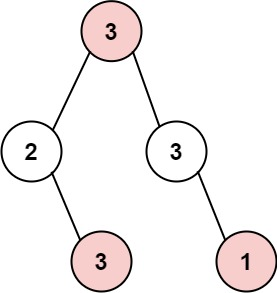
\includegraphics[width=0.2\linewidth]{images/lc0337_eg1}
\end{figure}
\item {\colorbox{CodeBackground}{\lstinline|root = [3,4,5,1,3,null,1] --> 9 (4 + 5)|}}
\begin{figure}[H]
\centering
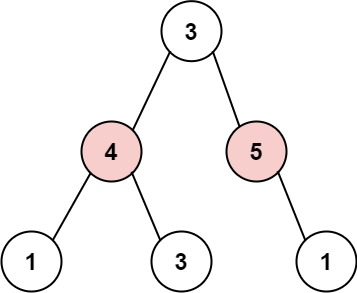
\includegraphics[width=0.25\linewidth]{images/lc0337_eg2}
\end{figure}
\end{itemize}

\subsection*{Solution - DP}
\begin{lstlisting}
int rob(TreeNode* root) {
  std::pair<int, int> result = RobTree(root);
  return std::max(result.first, result.second);
}

std::pair<int, int> RobTree(TreeNode* node) {
  if (!node) { return std::make_pair(0, 0); }
  auto left = RobTree(node->left);
  auto right = RobTree(node->right);
  // if we rob this node, we cannot rob its children
  int rob_curr = node->val + left.second + right.second;
  // if we do not rob this node, we take the maximum of robbing or not robbing its children
  int not_rob_curr = std::max(left.first, left.second) + std::max(right.first, right.second);
  return std::make_pair(rob_curr, not_rob_curr);
}
\end{lstlisting}

\subsection*{Related}
\begin{itemize}
\item \hyperref[lc0198]{LC 0198 - House Robber}
\item \hyperref[lc0213]{LC 0213 - House Robber II}
\item \hyperref[lc0337]{LC 0337 - House Robber III}
\end{itemize}

\section{LC 0055 - Jump Game}
You are given a {\colorbox{CodeBackground}{\lstinline|0|}}-indexed array of integers {\colorbox{CodeBackground}{\lstinline|nums|}} of length {\colorbox{CodeBackground}{\lstinline|n|}} ({\colorbox{CodeBackground}{\lstinline|n >= 1|}}. You are initially positioned at {\colorbox{CodeBackground}{\lstinline|nums[0]|}}. \\

Each element {\colorbox{CodeBackground}{\lstinline|nums[i]|}} represents the maximum length of a forward jump from index {\colorbox{CodeBackground}{\lstinline|i|}}. In other words, if you are at {\colorbox{CodeBackground}{\lstinline|nums[i]|}}, you can jump to any {\colorbox{CodeBackground}{\lstinline|nums[i + j]|}} where:
\begin{itemize}
	\item {\colorbox{CodeBackground}{\lstinline|0 <= j <= nums[i]|}}
	\item {\colorbox{CodeBackground}{\lstinline|i + j < n|}}
\end{itemize}

Return {\colorbox{CodeBackground}{\lstinline|true|}} if you can reach the last index, or {\colorbox{CodeBackground}{\lstinline|false|}} otherwise.\\

Examples:
\begin{itemize}
	\item {\colorbox{CodeBackground}{\lstinline|[2,3,1,1,4] --> True|}}
	\item {\colorbox{CodeBackground}{\lstinline|[3,2,1,0,4] --> False|}}
\end{itemize}

\subsection*{Solution - DP (Time Limit Exceeded)}\label{solution:lc0055_dp}
\begin{lstlisting}
bool canJump(std::vector<int>& nums) {
	int n = nums.size();
	// dp[i] = true if there is a path from num[0] to num[i]
	std::vector<bool> dp(n, false);
	dp[0] = true;
	for (int i = 1; i < n; ++i) {
		for (int j = 0; j < i; ++j) {
			if (dp[j] && j + nums[j] >= i) {
				dp[i] = true;
				break;
			}
		}
	}
	return dp.back();
}
\end{lstlisting}

\subsection*{Other Solutions}
\begin{itemize}
%	\item \hyperref[solution:lc0055_dp]{*DP}
	\item \hyperref[solution:lc0055_greedy]{Greedy}
\end{itemize}

\subsection*{Related}
\begin{itemize}
	\item \hyperref[lc0055]{LC 0055 - Jump Game}
	\item \hyperref[lc0045]{LC 0045 - Jump Game II}
\end{itemize}

\section{LC 0045 - Jump Game II}
You are given a {\colorbox{CodeBackground}{\lstinline|0|}}-indexed array of integers {\colorbox{CodeBackground}{\lstinline|nums|}} of length {\colorbox{CodeBackground}{\lstinline|n|}} ({\colorbox{CodeBackground}{\lstinline|n >= 1|}}. You are initially positioned at {\colorbox{CodeBackground}{\lstinline|nums[0]|}}. \\

Each element {\colorbox{CodeBackground}{\lstinline|nums[i]|}} represents the maximum length of a forward jump from index {\colorbox{CodeBackground}{\lstinline|i|}}. In other words, if you are at {\colorbox{CodeBackground}{\lstinline|nums[i]|}}, you can jump to any {\colorbox{CodeBackground}{\lstinline|nums[i + j]|}} where:
\begin{itemize}
	\item {\colorbox{CodeBackground}{\lstinline|0 <= j <= nums[i]|}}
	\item {\colorbox{CodeBackground}{\lstinline|i + j < n|}}
\end{itemize}

Return the minimum number of jumps to reach {\colorbox{CodeBackground}{\lstinline|nums[n - 1]|}}. \ul{It's guaranteed that you can reach {\colorbox{CodeBackground}{\lstinline|nums[n - 1]|}}.}\\

Examples:
\begin{itemize}
	\item {\colorbox{CodeBackground}{\lstinline|[2,3,1,1,4] --> 2 (2-->3-->4)|}}
	\item {\colorbox{CodeBackground}{\lstinline|[2,3,0,1,4] --> 2 (2-->3-->4)|}}
\end{itemize}

\subsection*{*Solution - DP}\label{solution:lc0045_dp}
\begin{lstlisting}
int jump(std::vector<int>& nums) {
	int n = nums.size();
	// dp[i] = min #jumps to reach num[i]
	std::vector<int> dp(n, std::numeric_limits<int>::max());
	dp[0] = 0;
	for (int i = 1; i < n; ++i) {
		for (int j = 0; j < i; ++j) {
			if (j + nums[j] >= i) { dp[i] = std::min(dp[i], dp[j] + 1); }
		}
	}
	return dp.back();
}
\end{lstlisting}

\subsection*{Other Solutions}
\begin{itemize}
%	\item \hyperref[solution:lc0045_dp]{*DP}
\item \hyperref[solution:lc0045_greedy]{Greedy}
\end{itemize}

\subsection*{Related}
\begin{itemize}
	\item \hyperref[lc0055]{LC 0055 - Jump Game}
	\item \hyperref[lc0045]{LC 0045 - Jump Game II}
\end{itemize}

\section{LC 0139 - Word Break}\label{lc0139}
Given a \ul{non-empty} string {\colorbox{CodeBackground}{\lstinline|s|}} and a dictionary of strings {\colorbox{CodeBackground}{\lstinline|wordDict|}}, return {\colorbox{CodeBackground}{\lstinline|true|}} if {\colorbox{CodeBackground}{\lstinline|s|}} can be segmented into a space-separated sequence of one or more dictionary words. Note that the same word in the dictionary may be reused \ul{multiple times} in the segmentation.\\

{\colorbox{CodeBackground}{\lstinline|s|}} and {\colorbox{CodeBackground}{\lstinline|wordDict[i]|}} consist of only \ul{lowercase English letters}.\\

Examples:
\begin{itemize}
	\item {\colorbox{CodeBackground}{\lstinline|s = "leetcode", wordDict = ["leet","code"] --> true|}}
	\item {\colorbox{CodeBackground}{\lstinline|s = "applepenapple", wordDict = ["apple","pen"] --> true|}}
	\item {\colorbox{CodeBackground}{\lstinline|s = "catsandog", wordDict = ["cats","dog","sand","and","cat"] --> false|}}
\end{itemize}

\subsection*{Solution - DP}
\begin{lstlisting}
bool wordBreak(std::string s, std::vector<std::string>& wordDict) {
  std::unordered_set<std::string> dict(wordDict.begin(), wordDict.end());
  // dp[i] = true if s.substr(0, i) can be broken into words
  std::vector<bool> dp(s.size() + 1, false);
  // base case: dp[0] = 0
  dp[0] = true;
  for (int i = 1; i <= s.size(); ++i) {
    for (int j = 0; j < i; ++j) {
      // s.substr(0, j) can be broken into words && s.substr(j, i - j) is in the dict
      if (dp[j] && dict.find(s.substr(j, i - j)) != dict.end()) {
        dp[i] = true;
        break;
      }
    }
  }
  return dp.back();
}
\end{lstlisting}

\section{LC 0300 - Longest Increasing Subsequence}\label{lc0300}
Given a \ul{non-empty} integer array {\colorbox{CodeBackground}{\lstinline|nums|}}, return the length of the \ul{longest strictly increasing subsequence}.\\

Examples:
\begin{itemize}
	\item {\colorbox{CodeBackground}{\lstinline|[10,9,2,5,3,7,101,18] --> 4 ([2, 3, 7, 101])|}}
	\item {\colorbox{CodeBackground}{\lstinline|[0,1,0,3,2,3] --> 4|}}
	\item {\colorbox{CodeBackground}{\lstinline|[7,7,7,7,7,7,7] --> 1|}}
\end{itemize}

\subsection*{Solution}
Be careful of the meaning of {\colorbox{CodeBackground}{\lstinline|dp[i]|}}. We don't return {\colorbox{CodeBackground}{\lstinline|dp.back()|}} here.
\begin{lstlisting}
int lengthOfLIS(std::vector<int>& nums) {
	// edge case
	if (nums.empty()) { return 0; }
	// dp[i] = length of LIS ending at nums[i]
	std::vector<int> dp(nums.size(), 1);
	int max_len = 1;
	for (int i = 1; i < nums.size(); ++i) {
		for (int j = 0; j < i; ++j) {
			if (nums[j] < nums[i]) { dp[i] = std::max(dp[i], dp[j] + 1); }
		}
		max_len = std::max(max_len, dp[i]);
	}
	return max_len;
}
\end{lstlisting}

\subsection*{Related - Subsequence}
\begin{itemize}
	\item \hyperref[lc0392]{LC 0392 - Is Subsequence}
	\item \hyperref[lc1143]{LC 1143 - Longest Common Subsequence}
	\item \hyperref[lc0300]{LC 0300 - Longest Increasing Subsequence}
	\item \hyperref[lc0516]{LC 0516 - Longest Palindromic Subsequence}
\end{itemize}

\section{LC 0053 - Maximum Sum of Subarray}
Given an \ul{non-empty} integer array {\colorbox{CodeBackground}{\lstinline|nums|}}, find the {\colorbox{CodeBackground}{\lstinline|subarray|}} with the largest sum, and return its sum.\\

Examples:
\begin{itemize}
	\item {\colorbox{CodeBackground}{\lstinline|nums = [-2,1,-3,4,-1,2,1,-5,4] --> 6 ([4,-1,2,1])|}}
	\item {\colorbox{CodeBackground}{\lstinline|nums = [1] --> 1|}}
	\item {\colorbox{CodeBackground}{\lstinline|nums = [5,4,-1,7,8] --> 23 ([5,4,-1,7,8])|}}
\end{itemize}

\subsection*{Solution - DP}\label{solution:lc0053_dp}
Be careful of the meaning of {\colorbox{CodeBackground}{\lstinline|dp[i]|}}. We don't return {\colorbox{CodeBackground}{\lstinline|dp.back()|}} here.
\begin{lstlisting}
int maxSubArray(std::vector<int>& nums) {
  // dp[i] - maximum sum of subarray in nums[0...i] which must end with nums[i]
  std::vector<int> dp(nums.size(), 0);
  dp[0] = nums[0];
  int max_sum = dp[0];
  for (int i = 1; i < nums.size(); ++i) {
    dp[i] = std::max(dp[i - 1] + nums[i], nums[i]);
    max_sum = std::max(max_sum, dp[i]);
  }
  return max_sum;
}
\end{lstlisting}

\subsection*{Other Solutions}
\begin{itemize}
\item \hyperref[solution:lc0053_greedy]{Greedy}
%\item \hyperref[solution:lc0053_dp]{DP}
\end{itemize}

\section{LC 0343 - Integer Break}
Given an integer {\colorbox{CodeBackground}{\lstinline|n (n >= 2)|}}, break it into the sum of {\colorbox{CodeBackground}{\lstinline|k|}} {\colorbox{CodeBackground}{\lstinline|(k >= 2)|}} positive integers that maximize the product of those integers. Return the maximum product you can get.

\subsection*{Solution - DP}
\begin{lstlisting}
int integerBreak(int n) {
  // dp[i] - max product you can get by breaking i into multiple positive integers
  std::vector<int> dp(n + 1, 0);
  // base case: dp[1] = 1
  dp[1] = 1;
  for (int i = 2; i <= n; ++i) {
    for (int j = 1; j < i; ++j) { dp[i] = std::max({dp[i], dp[j] * (i - j), j * (i - j)}); }
  }
  return dp[n];
}
\end{lstlisting}

\section{LC 0005 - Longest Palindromic Substring}
Given a \ul{non-empty} string {\colorbox{CodeBackground}{\lstinline|s|}}, return the longest \ul{palindromic substring} in {\colorbox{CodeBackground}{\lstinline|s|}}.\\

Examples:
\begin{itemize}
	\item {\colorbox{CodeBackground}{\lstinline|"babad" --> "bab"\ \ or "aba"|}}
	\item {\colorbox{CodeBackground}{\lstinline|"cbbd" --> "bb"|}}
\end{itemize}

{\colorbox{CodeBackground}{\lstinline|s|}} consist of only \ul{digits} and \ul{English letters}.\\

\subsection*{Solution - DP}\label{solution:lc0005_dp}
\begin{lstlisting}
std::string longestPalindrome(std::string s) {
	int n = s.size();
	// edge case
	if (n <= 1) { return s; }
	// dp[i][j] = true if s[i...j] is a palindrome
	std::vector<std::vector<bool>> dp(n, std::vector<bool>(n, false));
	int begin = 0;
	int max_len = 1;
	// substrings of length 1
	for (int i = 0; i < n; ++i) { dp[i][i] = true; }
	// substrings of length 2
	for (int i = 0; i < n - 1; ++i) {
		if (s[i] == s[i + 1]) {
			dp[i][i + 1] = true;
			begin = i;
			max_len = 2;
		}
	}
	// substrings of length > 2
	for (int len = 3; len <= n; ++len) {
		for (int i = 0; i < n - len + 1; ++i) {
			int j = i + len - 1;
			if (s[i] == s[j] && dp[i + 1][j - 1]) {
				dp[i][j] = true;
				begin = i;
				max_len = len;
			}
		}
	}
	return s.substr(begin, max_len);
}
\end{lstlisting}

\subsection*{Other Solutions}
\begin{itemize}
	\item \hyperref[solution:lc0005_expand_around_center]{Expand Around Center}
	%	\item \hyperref[solution:lc0005_dp]{DP}
\end{itemize}

\subsection*{Related - Palindrome}
\begin{itemize}
	\item \hyperref[lc0125]{LC 0125 - Valid Palindrome}
 	\item \hyperref[lc0680]{LC 0680 - Valid Palindrome II}
	\item \hyperref[lc0647]{LC 0647 - Palindromic Substrings}
	\item \hyperref[lc0005]{LC 0005 - Longest Palindromic Substring}
	\item \hyperref[lc0516]{LC 0516 - Longest Palindromic Subsequence}
\end{itemize}

\section{LC 0516 - Longest Palindromic Subsequence}\label{lc0516}
Given a \ul{non-empty} string {\colorbox{CodeBackground}{\lstinline|s|}}, find the \ul{longest palindromic subsequence}'s length in {\colorbox{CodeBackground}{\lstinline|s|}}. \\

Examples:
\begin{itemize}
	\item {\colorbox{CodeBackground}{\lstinline|s = "bbbab" --> 4|}}
	\item {\colorbox{CodeBackground}{\lstinline|s = "cbbd" --> 2|}}
\end{itemize}

{\colorbox{CodeBackground}{\lstinline|s|}} consists only of \ul{lowercase English letters}.\\

\subsection*{Solution - DP}
\begin{lstlisting}
int longestPalindromeSubseq(std::string s) {
	int n = s.length();
	// dp[i][j] = length of longest palindromic subsequence in s[i...j]
	std::vector<std::vector<int>> dp(n, std::vector<int>(n, 0));
	for (int i = 0; i < n; ++i) { dp[i][i] = 1; }
	for (int len = 2; len <= n; ++len) {
		for (int begin = 0; begin <= n - len; ++begin) {
			int end = begin + len - 1;
			if (s[begin] == s[end]) {
				dp[begin][end] = 2 + (len == 2 ? 0 : dp[begin + 1][end - 1]);
			} else {
				dp[begin][end] = std::max(dp[begin + 1][end], dp[begin][end - 1]);
			}
		}
	}
	return dp[0][n - 1];
}
\end{lstlisting}

\subsection*{Related - Subsequence}
\begin{itemize}
	\item \hyperref[lc0392]{LC 0392 - Is Subsequence}
	\item \hyperref[lc1143]{LC 1143 - Longest Common Subsequence}
	\item \hyperref[lc0300]{LC 0300 - Longest Increasing Subsequence}
	\item \hyperref[lc0516]{LC 0516 - Longest Palindromic Subsequence}
\end{itemize}

\subsection*{Related - Palindrome}
\begin{itemize}
	\item \hyperref[lc0125]{LC 0125 - Valid Palindrome}
 	\item \hyperref[lc0680]{LC 0680 - Valid Palindrome II}
	\item \hyperref[lc0647]{LC 0647 - Palindromic Substrings}
	\item \hyperref[lc0005]{LC 0005 - Longest Palindromic Substring}
	\item \hyperref[lc0516]{LC 0516 - Longest Palindromic Subsequence}
\end{itemize}

\section{LC 1143 - Longest Common Subsequence}\label{lc1143}
\begin{tcolorbox}
\begin{itemize}
\item Given two \ul{sequences} (array, string, linked list, etc.), find their \ul{longest common subsequence}.
\end{itemize}
\end{tcolorbox}
Given two \ul{non-empty} strings {\colorbox{CodeBackground}{\lstinline|text1|}} and {\colorbox{CodeBackground}{\lstinline|text2|}}, return the length of their \ul{longest common subsequence}. If there is no common subsequence, return {\colorbox{CodeBackground}{\lstinline|0|}}.\\

{\colorbox{CodeBackground}{\lstinline|text1|}} and {\colorbox{CodeBackground}{\lstinline|text2|}} consist of only \ul{lowercase English characters}.

Examples:
\begin{itemize}
	\item {\colorbox{CodeBackground}{\lstinline|text1 = "abcde", text2 = "ace"  --> 3|}}
	\item {\colorbox{CodeBackground}{\lstinline|text1 = "abc", text2 = "abc" --> 3|}}
	\item {\colorbox{CodeBackground}{\lstinline|text1 = "abc", text2 = "def" --> 0|}}
\end{itemize}

\subsection*{Solution - DP}\label{solution:lc1143_dp}
\begin{lstlisting}
int longestCommonSubsequence(std::string str1, std::string str2) {
	// dp[i][j] = length of LCS of str1.substr(0, i) and str2.substr(0, j)
	std::vector<std::vector<int>> dp(str1.size() + 1, std::vector<int>(str2.size() + 1, 0));
	for (int i = 1; i <= str1.size(); i++) {
		for (int j = 1; j <= str2.size(); j++) {
			if (str1[i - 1] == str2[j - 1]) {
				dp[i][j] = dp[i - 1][j - 1] + 1;
			} else {
				dp[i][j] = std::max(dp[i - 1][j], dp[i][j - 1]);
			}
		}
	}
	return dp[str1.size()][str2.size()];
}
\end{lstlisting}

\subsection*{Related - Subsequence}
\begin{itemize}
	\item \hyperref[lc0392]{LC 0392 - Is Subsequence}
	\item \hyperref[lc1143]{LC 1143 - Longest Common Subsequence}
	\item \hyperref[lc0300]{LC 0300 - Longest Increasing Subsequence}
	\item \hyperref[lc0516]{LC 0516 - Longest Palindromic Subsequence}
\end{itemize}

\section{LC 0097 - Interleaving String}\label{lc0097}
Given strings {\colorbox{CodeBackground}{\lstinline|s1|}}, {\colorbox{CodeBackground}{\lstinline|s2|}}, and {\colorbox{CodeBackground}{\lstinline|s3|}}, find whether {\colorbox{CodeBackground}{\lstinline|s3|}} is formed by an \ul{interleaving} of {\colorbox{CodeBackground}{\lstinline|s1|}} and {\colorbox{CodeBackground}{\lstinline|s2|}}.\\

An interleaving of two strings {\colorbox{CodeBackground}{\lstinline|s|}} and {\colorbox{CodeBackground}{\lstinline|t|}} is a configuration where {\colorbox{CodeBackground}{\lstinline|s|}} and {\colorbox{CodeBackground}{\lstinline|t|}} are divided into {\colorbox{CodeBackground}{\lstinline|n|}} and {\colorbox{CodeBackground}{\lstinline|m|}} substrings respectively, such that:
\begin{itemize}
	\item $s = s_1 + s_2 + \dots + s_n$
	\item $t = t_1 + t_2 + \dots + t_m$
	\item $|n - m| <= 1$
	\item The interleaving is $s_1 + t_1 + s_2 + t_2 + s_3 + t_3 + \dots$ or $t_1 + s_1 + t_2 + s_2 + t_3 + s_3 + \dots$
\end{itemize}

{\colorbox{CodeBackground}{\lstinline|s1|}}, {\colorbox{CodeBackground}{\lstinline|s2|}}, and {\colorbox{CodeBackground}{\lstinline|s3|}} consist of \ul{lowercase English letters}.\\

Examples:
\begin{itemize}
	\item {\colorbox{CodeBackground}{\lstinline|s1 = "aabcc", s2 = "dbbca", s3 = "aadbbcbcac"; --> true ("aa-dbbc-bc-a-c")|}}
	\item {\colorbox{CodeBackground}{\lstinline|s1 = "aabcc", s2 = "dbbca", s3 = "aadbbbaccc"; --> false|}}
	\item {\colorbox{CodeBackground}{\lstinline|s1 = "", s2 = "", s3 = ""; --> true|}}
\end{itemize}

\subsection*{Solution - DP}
\begin{lstlisting}
bool isInterleave(std::string s1, std::string s2, std::string s3) {
	int m = s1.size();
	int n = s2.size();
	int l = s3.size();
	if (n + m != l) { return false; }
	// dp[i][j] = true if s1.substr(0,i) and s2.substr(0,j) can interleave to s3.substr(0,i+j)
	std::vector<std::vector<bool>> dp(m + 1, std::vector<bool>(n + 1, false));
	dp[0][0] = true;
	for (int i = 1; i <= m; ++i) { dp[i][0] = dp[i - 1][0] && s1[i - 1] == s3[i - 1]; }
	for (int j = 1; j <= n; ++j) { dp[0][j] = dp[0][j - 1] && s2[j - 1] == s3[j - 1]; }
	for (int i = 1; i <= m; ++i) {
		for (int j = 1; j <= n; ++j) {
			dp[i][j] = (dp[i - 1][j] && s1[i - 1] == s3[i + j - 1])
								  || (dp[i][j - 1] && s2[j - 1] == s3[i + j - 1]);
		}
	}
	return dp[m][n];
}
\end{lstlisting}

\subsection*{Related - Interleaving}
\begin{itemize}
\item \hyperref[lc0097]{LC 0097 - Interleaving String}
\item \hyperref[lc1768]{LC 1768 - Merge Strings Alternately}
\end{itemize}

\section{LC 0072 - Edit Distance (Levenshtein Distance)}
\begin{tcolorbox}
\begin{itemize}
\item Levenshtein Distance: The minimum number of single-character edits (insertions, deletions or substitutions) required to change one string into another string.
\end{itemize}
\end{tcolorbox}

Given two strings {\colorbox{CodeBackground}{\lstinline|word1|}} and {\colorbox{CodeBackground}{\lstinline|word2|}}, return the minimum number of operations required to convert {\colorbox{CodeBackground}{\lstinline|word1|}} to {\colorbox{CodeBackground}{\lstinline|word2|}}.\\

You have the following three operations permitted on a word:
\begin{itemize}
	\item Insert a character;
	\item Delete a character;
	\item Replace a character;
\end{itemize}

{\colorbox{CodeBackground}{\lstinline|word1|}} and {\colorbox{CodeBackground}{\lstinline|word2|}} consist of \ul{lowercase English letters}.\\

Examples:
\begin{itemize}
	\item {\colorbox{CodeBackground}{\lstinline|word1 = "horse", word2 = "ros"; --> 3|}}
	\item {\colorbox{CodeBackground}{\lstinline|word1 = "intention", word2 = "execution"; --> 5|}}
\end{itemize}

\subsection*{Solution - DP}
\begin{lstlisting}
int minDistance(std::string word1, std::string word2) {
  int m = word1.size();
  int n = word2.size();
  // dp[i][j] = min edit distance between word1.substr(0, i) and word2.substr(0, j)
  std::vector<std::vector<int>> dp(m + 1, std::vector<int>(n + 1, 0));
  dp[0][0] = 0;
  for (int i = 1; i <= m; ++i) { dp[i][0] = i; }
  for (int j = 1; j <= n; ++j) { dp[0][j] = j; }
  for (int i = 1; i <= m; ++i) {
    for (int j = 1; j <= n; ++j) {
      if (word1[i - 1] == word2[j - 1]) {
        dp[i][j] = dp[i - 1][j - 1];
      } else {
        dp[i][j] =
            1
            + std::min(
                {/* [Deletion] delete the last character of word1.substr(0, i) before the
                    transformation from word1.sbustr(0, i - 1) to word2.substr(0, j) */
                 dp[i - 1][j],
                 /* [Insertion] append the last character of word2.substr(0, j) to
                    word2.substr(0, j - 1) after the transformation from word1.sbustr(0, i)
                    to word2.substr(0, j - 1) */
                 dp[i][j - 1],
                 /* [Substitution] replace the last character of word1.substr(0, i) with the
                    last character of word2.substr(0, j) after the transformation from
                    word1.sbustr(0, i - 1) to word2.substr(0, j - 1) */
                 dp[i - 1][j - 1]});
      }
    }
  }
  return dp[m][n];
}
\end{lstlisting}

\section{LC 0096 - Unique Binary Search Trees}
Given an integer {\colorbox{CodeBackground}{\lstinline|n|}} ({\colorbox{CodeBackground}{\lstinline|n >= 1|}}), return the number of structurally unique BST's (binary search trees) which has exactly {\colorbox{CodeBackground}{\lstinline|n|}} nodes of unique values from {\colorbox{CodeBackground}{\lstinline|1|}} to {\colorbox{CodeBackground}{\lstinline|n|}}.

\begin{itemize}
\item {\colorbox{CodeBackground}{\lstinline|n = 3 --> 5|}}
\begin{figure}[H]
\centering
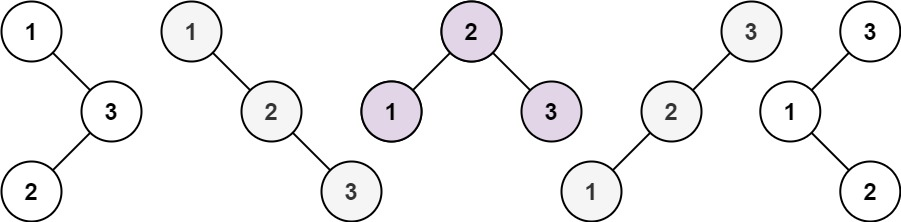
\includegraphics[width=0.65\linewidth]{images/lc0096_eg}
\end{figure}
\item {\colorbox{CodeBackground}{\lstinline|n = 1 --> 1|}}
\end{itemize}

\subsection*{Solution - DP}\label{solution:lc0096_dp}
\begin{lstlisting}
int numTrees(int n) {
  // dp[i] - number of unique BSTs with i nodes
  std::vector<int> dp(n + 1, 0);
  dp[0] = 1;
  dp[1] = 1;
  for (int nodes = 2; nodes <= n; ++nodes) {
    for (int root = 1; root <= nodes; ++root) {
      dp[nodes] += dp[root - 1] * dp[nodes - root];
    }
  }
  return dp[n];
}
\end{lstlisting}

\subsection*{Other Solutions}
\begin{itemize}
\item \hyperref[solution:lc0096_recursion]{Recursion}
%\item \hyperref[solution:lc0096_dp]{DP}
\end{itemize}

\section{LC 0416 - Partition Equal Subset Sum}\label{lc0416}
{\hyperref[subsubsec:01_knapsack_oj_problems]{[0/1 Knapsack Problem]}} \\

Given an \ul{non-empty} integer array {\colorbox{CodeBackground}{\lstinline|nums|}}, return {\colorbox{CodeBackground}{\lstinline|true|}} if you can partition the array into two subsets such that the sum of the elements in both subsets is equal or {\colorbox{CodeBackground}{\lstinline|false|}} otherwise.\\

Examples:
\begin{itemize}
\item {\colorbox{CodeBackground}{\lstinline|nums = [1,5,11,5] --> true|}}\\
The array can be partitioned as {\colorbox{CodeBackground}{\lstinline|[1, 5, 5]|}} and {\colorbox{CodeBackground}{\lstinline|[11]|}}.
\item {\colorbox{CodeBackground}{\lstinline|nums = [1,2,3,5] --> false|}}\\
The array cannot be partitioned into equal sum subsets.
\end{itemize}

\subsection*{Solution 1 - 2D DP Table (Item First, Capacity Second)}
\begin{lstlisting}
bool canPartition(std::vector<int>& nums) {
  int sum = std::accumulate(nums.begin(), nums.end(), 0);
  if (sum % 2 != 0) { return false; }
  int target = sum / 2;
  // dp[i][j] = true if j can be achieved by summing up some of the first i numbers
  std::vector<std::vector<bool>> dp(nums.size() + 1, std::vector<bool>(target + 1, false));
  // base case: dp[i][0] = true
  for (int i = 0; i <= nums.size(); ++i) { dp[i][0] = true; }
  for (int i = 1; i <= nums.size(); ++i) {
    for (int j = 1; j <= target; ++j) {
      if (j < nums[i - 1]) {
        dp[i][j] = dp[i - 1][j];
      } else {
        dp[i][j] = dp[i - 1][j] || dp[i - 1][j - nums[i - 1]];
      }
    }
  }
  return dp[nums.size()][target];
}
\end{lstlisting}

\subsection*{Solution 2 - 2D DP Table (Capacity First, Item Second)}
\begin{lstlisting}
bool canPartition(std::vector<int>& nums) {
  int sum = std::accumulate(nums.begin(), nums.end(), 0);
  if (sum % 2 != 0) { return false; }
  int target = sum / 2;
  // dp[i][j] = true if j can be achieved by summing up some of the first i numbers
  std::vector<std::vector<bool>> dp(nums.size() + 1, std::vector<bool>(target + 1, false));
  // base case: dp[i][0] = true
  for (int i = 0; i <= nums.size(); ++i) { dp[i][0] = true; }
  for (int j = 1; j <= target; ++j) {
    for (int i = 1; i <= nums.size(); ++i) {
      if (j < nums[i - 1]) {
        dp[i][j] = dp[i - 1][j];
      } else {
        dp[i][j] = dp[i - 1][j] || dp[i - 1][j - nums[i - 1]];
      }
    }
  }
  return dp[nums.size()][target];
}
\end{lstlisting}

\subsection*{Solution 3 - 1D DP Vector (Item First, Capacity Second)}
\begin{lstlisting}
bool canPartition(std::vector<int>& nums) {
  int sum = std::accumulate(nums.begin(), nums.end(), 0);
  if (sum % 2 != 0) { return false; }
  int target = sum / 2;
  // dp[i] = true if i can be achieved by summing up some of the numbers
  std::vector<bool> dp(target + 1, false);
  // base case: dp[0] = true
  dp[0] = true;
  for (int num : nums) {
    for (int i = target; i >= num; --i) {
      if (dp[i - num]) { dp[i] = true; }
    }
  }
  return dp[target];
}
\end{lstlisting}

\section{LC 1049 - Last Stone Weight II}\label{lc1049}
{\hyperref[subsubsec:01_knapsack_oj_problems]{[0/1 Knapsack Problem]}} \\

You are given a \ul{non-empty} array of integers {\colorbox{CodeBackground}{\lstinline|stones|}} where {\colorbox{CodeBackground}{\lstinline|stones[i]|}} is the weight of the {\colorbox{CodeBackground}{\lstinline|i|}}th stone ({\colorbox{CodeBackground}{\lstinline|stones[i] >= 1|}}).\\

We are playing a game with the stones. On each turn, we choose any two stones and smash them together. Suppose the stones have weights {\colorbox{CodeBackground}{\lstinline|x|}} and {\colorbox{CodeBackground}{\lstinline|y|}} with {\colorbox{CodeBackground}{\lstinline|x <= y|}}. The result of this smash is:
\begin{itemize}
\item If {\colorbox{CodeBackground}{\lstinline|x == y|}}, both stones are destroyed, and
\item If {\colorbox{CodeBackground}{\lstinline|x != y|}}, the stone of weight {\colorbox{CodeBackground}{\lstinline|x|}} is destroyed, and the stone of weight {\colorbox{CodeBackground}{\lstinline|y|}} has new weight {\colorbox{CodeBackground}{\lstinline|y - x|}}.
\end{itemize}

At the end of the game, there is \ul{at most one stone left}.\\

Return the smallest possible weight of the left stone. If there are no stones left, return {\colorbox{CodeBackground}{\lstinline|0|}}.\\

Examples:
\begin{itemize}
\item {\colorbox{CodeBackground}{\lstinline|stones = [2,7,4,1,8,1] --> 1|}}\\
We can combine {\colorbox{CodeBackground}{\lstinline|2|}} and {\colorbox{CodeBackground}{\lstinline|4|}} to get {\colorbox{CodeBackground}{\lstinline|2|}}, so the array converts to {\colorbox{CodeBackground}{\lstinline|[2,7,1,8,1]|}} then,\\
we can combine {\colorbox{CodeBackground}{\lstinline|7|}} and {\colorbox{CodeBackground}{\lstinline|8|}} to get {\colorbox{CodeBackground}{\lstinline|1|}}, so the array converts to {\colorbox{CodeBackground}{\lstinline|[2,1,1,1]|}} then,\\
we can combine {\colorbox{CodeBackground}{\lstinline|2|}} and {\colorbox{CodeBackground}{\lstinline|1|}} to get {\colorbox{CodeBackground}{\lstinline|1|}}, so the array converts to {\colorbox{CodeBackground}{\lstinline|[1,1,1]|}} then,\\
we can combine {\colorbox{CodeBackground}{\lstinline|1|}} and {\colorbox{CodeBackground}{\lstinline|1|}} to get {\colorbox{CodeBackground}{\lstinline|0|}}, so the array converts to {\colorbox{CodeBackground}{\lstinline|[1]|}}, then that's the optimal value.
\item {\colorbox{CodeBackground}{\lstinline|stones = [31,26,33,21,40] --> 5|}}
\end{itemize}

\subsection*{Solution 1 - 2D DP Table (Item First, Capacity Second)}
\begin{lstlisting}
int lastStoneWeightII(std::vector<int>& stones) {
  int sum = std::accumulate(stones.begin(), stones.end(), 0);
  int target = sum / 2;
  // dp[i][j] - the maximum weight using the first i stones with a capacity of j
  std::vector<std::vector<int>> dp(stones.size() + 1, std::vector<int>(target + 1, 0));
  for (int i = 1; i <= stones.size(); ++i) {
    for (int j = 0; j <= target; ++j) {
      if (stones[i - 1] > j) {
        dp[i][j] = dp[i - 1][j];
      } else {
        dp[i][j] = std::max(dp[i - 1][j], dp[i - 1][j - stones[i - 1]] + stones[i - 1]);
      }
    }
  }
  return sum - 2 * dp[stones.size()][target];
}
\end{lstlisting}

\subsection*{Solution 2 - 2D DP Table (Capacity First, Item Second)}
\begin{lstlisting}
int lastStoneWeightII(std::vector<int>& stones) {
  int sum = std::accumulate(stones.begin(), stones.end(), 0);
  int target = sum / 2;
  // dp[i][j] - the maximum weight using the first i stones with a capacity of j
  std::vector<std::vector<int>> dp(stones.size() + 1, std::vector<int>(target + 1, 0));
  for (int j = 0; j <= target; ++j) {
    for (int i = 1; i <= stones.size(); ++i) {
      if (stones[i - 1] > j) {
        dp[i][j] = dp[i - 1][j];
      } else {
        dp[i][j] = std::max(dp[i - 1][j], dp[i - 1][j - stones[i - 1]] + stones[i - 1]);
      }
    }
  }
  return sum - 2 * dp[stones.size()][target];
}
\end{lstlisting}

\subsection*{Solution 3 - 1D DP Table (Item First, Capacity Second)}
\begin{lstlisting}
int lastStoneWeightII(std::vector<int>& stones) {
  int sum = std::accumulate(stones.begin(), stones.end(), 0);
  int target = sum / 2;
  // dp[i] - the maximum weight using the first i stones
  std::vector<int> dp(target + 1, 0);
  for (int stone : stones) {
    for (int j = target; j >= stone; --j) { dp[j] = std::max(dp[j], dp[j - stone] + stone); }
  }
  return sum - 2 * dp[target];
}
\end{lstlisting}

\section{LC 0494 - Target Sum}\label{lc0494}
{\hyperref[subsubsec:01_knapsack_oj_problems]{[0/1 Knapsack Problem]}} \\

You are given an \ul{non-empty} \ul{non-negative} integer array {\colorbox{CodeBackground}{\lstinline|nums|}} and an integer {\colorbox{CodeBackground}{\lstinline|target|}}.\\

You want to build an expression out of {\colorbox{CodeBackground}{\lstinline|nums|}} by adding one of the symbols {\colorbox{CodeBackground}{\lstinline|'+'|}} and {\colorbox{CodeBackground}{\lstinline|'-'|}} before each integer in {\colorbox{CodeBackground}{\lstinline|nums|}} and then concatenate all the integers.\\

For example, if {\colorbox{CodeBackground}{\lstinline|nums = [2, 1]|}}, you can add a {\colorbox{CodeBackground}{\lstinline|'+'|}} before {\colorbox{CodeBackground}{\lstinline|2|}} and a {\colorbox{CodeBackground}{\lstinline|'-'|}} before {\colorbox{CodeBackground}{\lstinline|1|}} and concatenate them to build the expression {\colorbox{CodeBackground}{\lstinline|"+2-1"|}}. Return the number of different expressions that you can build, which evaluates to {\colorbox{CodeBackground}{\lstinline|target|}}.\\

Examples:
\begin{itemize}
\item {\colorbox{CodeBackground}{\lstinline|nums = [1,1,1,1,1], target = 3 --> 5|}}\\
There are {\colorbox{CodeBackground}{\lstinline|5|}} ways to assign symbols to make the sum of {\colorbox{CodeBackground}{\lstinline|nums|}} be target {\colorbox{CodeBackground}{\lstinline|3|}}.\\
{\colorbox{CodeBackground}{\lstinline|-1 + 1 + 1 + 1 + 1 = 3|}} \\
{\colorbox{CodeBackground}{\lstinline|+1 - 1 + 1 + 1 + 1 = 3|}} \\
{\colorbox{CodeBackground}{\lstinline|+1 + 1 - 1 + 1 + 1 = 3|}} \\
{\colorbox{CodeBackground}{\lstinline|+1 + 1 + 1 - 1 + 1 = 3|}} \\
{\colorbox{CodeBackground}{\lstinline|+1 + 1 + 1 + 1 - 1 = 3|}}
\item {\colorbox{CodeBackground}{\lstinline|nums = [1], target = 1 --> 1|}}
\end{itemize}

\subsection*{Solution - DP}
\begin{lstlisting}
int findTargetSumWays(std::vector<int>& nums, int target) {
  int sum = std::accumulate(nums.begin(), nums.end(), 0);
  if (std::abs(target) > sum) { return 0; }
  if ((target + sum) % 2 == 1) { return 0; }
  int capacity = (target + sum) / 2;
  std::vector<int> dp(capacity + 1, 0);
  dp[0] = 1;
  for (int num : nums) {
    for (int i = capacity; i >= num; --i) { dp[i] += dp[i - num]; }
  }
  return dp[capacity];
}
\end{lstlisting}

\section{LC 0474 - Ones and Zeroes}\label{lc0474}
{\hyperref[subsubsec:01_knapsack_oj_problems]{[0/1 Knapsack Problem]}} \\

You are given a \ul{non-empty} array of \ul{non-empty} binary strings {\colorbox{CodeBackground}{\lstinline|strs|}} and two integers {\colorbox{CodeBackground}{\lstinline|m|}} and {\colorbox{CodeBackground}{\lstinline|n|}} ({\colorbox{CodeBackground}{\lstinline|m, n >= 1|}}).\\

Return the size of the largest \ul{subset} of {\colorbox{CodeBackground}{\lstinline|strs|}} such that there are at most {\colorbox{CodeBackground}{\lstinline|m|}} {\colorbox{CodeBackground}{\lstinline|0|}}s and {\colorbox{CodeBackground}{\lstinline|n|}} {\colorbox{CodeBackground}{\lstinline|1|}}s in the subset.\\

Examples:
\begin{itemize}
\item {\colorbox{CodeBackground}{\lstinline|strs = ["10","0001","111001","1","0"], m = 5, n = 3 --> 4|}}\\
The largest subset with at most {\colorbox{CodeBackground}{\lstinline|5|}} {\colorbox{CodeBackground}{\lstinline|0|}}s and {\colorbox{CodeBackground}{\lstinline|3|}} {\colorbox{CodeBackground}{\lstinline|1|}}s is {\colorbox{CodeBackground}{\lstinline|\{"10", "0001", "1", "0"\}|}}, so the answer is {\colorbox{CodeBackground}{\lstinline|4|}}.
\item {\colorbox{CodeBackground}{\lstinline|strs = ["10","0","1"], m = 1, n = 1 --> 2|}}\\
The largest subset is {\colorbox{CodeBackground}{\lstinline|\{"0", "1"\}|}}, so the answer is {\colorbox{CodeBackground}{\lstinline|2|}}.
\end{itemize}

\subsection*{Solution - DP}
\begin{lstlisting}
int findMaxForm(std::vector<std::string>& strs, int m, int n) {
  std::vector<std::vector<int>> dp(m + 1, std::vector<int>(n + 1, 0));
  for (std::string str : strs) {
    int num_zeros = std::count(str.begin(), str.end(), '0');
    int num_ones = std::count(str.begin(), str.end(), '1');
    for (int i = m; i >= num_zeros; --i) {
      for (int j = n; j >= num_ones; --j) {
        dp[i][j] = std::max(dp[i][j], dp[i - num_zeros][j - num_ones] + 1);
      }
    }
  }
  return dp[m][n];
}
\end{lstlisting}

\section{LC 0322 - Coin Change}\label{lc0322}
{\hyperref[subsubsec:unbounded_knapsack_oj_problems]{[Unbounded Knapsack Problem]}} \\

You are given a \ul{non-empty} integer array {\colorbox{CodeBackground}{\lstinline|coins|}} ({\colorbox{CodeBackground}{\lstinline|coin[i] >= 1|}}) representing coins of different denominations and an integer {\colorbox{CodeBackground}{\lstinline|amount|}} ({\colorbox{CodeBackground}{\lstinline|amount >= 0|}}) representing a total amount of money. Return the \ul{fewest number of coins} that you need to make up that amount. If that amount of money cannot be made up by any combination of the coins, return {\colorbox{CodeBackground}{\lstinline|-1|}}.\\

Examples:
\begin{itemize}
	\item {\colorbox{CodeBackground}{\lstinline|coins = [1,2,5], amount = 11 --> 3 (5 + 5  + 1)|}}
	\item {\colorbox{CodeBackground}{\lstinline|coins = [2], amount = 3 --> -1|}}
	\item {\colorbox{CodeBackground}{\lstinline|coins = [1], amount = 0 --> 0|}}
\end{itemize}

\subsection*{Solution 1 - 2D DP Table (Item First, Capacity Second)}
\begin{lstlisting}
int coinChange(std::vector<int>& coins, int amount) {
  // dp[i][j] - min number of the first i coins to make up amount j
  std::vector<std::vector<int>> dp(coins.size() + 1,
                                   std::vector<int>(amount + 1, amount + 1));
  // base case: dp[i][0] = 0
  for (int i = 0; i <= coins.size(); ++i) { dp[i][0] = 0; }
  for (int i = 1; i <= coins.size(); ++i) {
    for (int j = 1; j <= amount; ++j) {
      if (j < coins[i - 1]) {
        dp[i][j] = dp[i - 1][j];
      } else {
        dp[i][j] = std::min(dp[i - 1][j], dp[i][j - coins[i - 1]] + 1);
      }
    }
  }
  return dp[coins.size()][amount] == amount + 1 ? -1 : dp[coins.size()][amount];
}
\end{lstlisting}

\subsection*{Solution 2 - 2D DP Table (Capacity First, Item Second)}
\begin{lstlisting}
int coinChange(std::vector<int>& coins, int amount) {
  // dp[i][j] - min number of the first i coins to make up amount j
  std::vector<std::vector<int>> dp(coins.size() + 1,
                                   std::vector<int>(amount + 1, amount + 1));
  // base case: dp[i][0] = 0
  for (int i = 0; i <= coins.size(); ++i) { dp[i][0] = 0; }
  for (int j = 1; j <= amount; ++j) {
    for (int i = 1; i <= coins.size(); ++i) {
      if (j < coins[i - 1]) {
        dp[i][j] = dp[i - 1][j];
      } else {
        dp[i][j] = std::min(dp[i - 1][j], dp[i][j - coins[i - 1]] + 1);
      }
    }
  }
  return dp[coins.size()][amount] == amount + 1 ? -1 : dp[coins.size()][amount];
}
\end{lstlisting}

\subsection*{Solution 3 - 1D DP Vector (Item First, Capacity Second)}
\begin{lstlisting}
int coinChange(std::vector<int>& coins, int amount) {
  // dp[i] = min number of coins to make up amount i
  std::vector<int> dp(amount + 1, amount + 1);
  // base case: dp[0] = 0
  dp[0] = 0;
  for (int coin : coins) {
    for (int i = coin; i <= amount; ++i) { dp[i] = std::min(dp[i], dp[i - coin] + 1); }
  }
  return dp[amount] == amount + 1 ? -1 : dp[amount];
}
\end{lstlisting}

\subsection*{Solution 4 - 1D DP Vector (Capacity First, Item Second)}
\begin{lstlisting}
int coinChange(std::vector<int>& coins, int amount) {
  // dp[i] = min number of coins to make up amount i
  std::vector<int> dp(amount + 1, amount + 1);
  // base case: dp[0] = 0
  dp[0] = 0;
  for (int i = 1; i <= amount; ++i) {
    for (int coin : coins) {
      if (i >= coin) { dp[i] = std::min(dp[i], dp[i - coin] + 1); }
    }
  }
  return dp[amount] == amount + 1 ? -1 : dp[amount];
}
\end{lstlisting}

\subsection*{Related}
\begin{itemize}
\item \hyperref[lc0322]{LC 0322 - Coin Change}
\item \hyperref[lc0518]{LC 0518 - Coin Change II}
\end{itemize}

\section{LC 0518 - Coin Change II}\label{lc0518}
{\hyperref[subsubsec:unbounded_knapsack_oj_problems]{[Unbounded Knapsack Problem]}} \\

You are given a \ul{non-empty} integer array {\colorbox{CodeBackground}{\lstinline|coins|}} ({\colorbox{CodeBackground}{\lstinline|coin[i] >= 1|}}) representing coins of different denominations and an integer {\colorbox{CodeBackground}{\lstinline|amount|}} ({\colorbox{CodeBackground}{\lstinline|amount >= 0|}}) representing a total {\colorbox{CodeBackground}{\lstinline|amount|}} of money. Return the \ul{number of combinations} that make up that amount. If that amount of money cannot be made up by any combination of the coins, return {\colorbox{CodeBackground}{\lstinline|0|}}.\\

Examples:
\begin{itemize}
\item {\colorbox{CodeBackground}{\lstinline|coins = [1,2,5], amount = 5 --> 4|}}\\
There are four ways to make up the amount:\\
{\colorbox{CodeBackground}{\lstinline|5=5|}} \\
{\colorbox{CodeBackground}{\lstinline|5=2+2+1|}} \\
{\colorbox{CodeBackground}{\lstinline|5=2+1+1+1|}} \\
{\colorbox{CodeBackground}{\lstinline|5=1+1+1+1+1|}}
\item {\colorbox{CodeBackground}{\lstinline|coins = [2], amount = 3 --> 0|}}\\
The amount of {\colorbox{CodeBackground}{\lstinline|3|}} cannot be made up just with coins of {\colorbox{CodeBackground}{\lstinline|2|}}.
\item {\colorbox{CodeBackground}{\lstinline|coins = [10], amount = 10 --> 1|}}
\end{itemize}

\subsection*{Solution 1 - 2D DP Table (Item First, Capacity Second)}
\begin{lstlisting}
int change(int amount, std::vector<int>& coins) {
  // dp[i][j] - number of combinations to make up amount j using the first i coins
  std::vector<std::vector<int>> dp(coins.size() + 1, std::vector<int>(amount + 1, 0));
  // base case: dp[i][0] = 1
  for (int i = 0; i <= coins.size(); ++i) { dp[i][0] = 1; }
  for (int i = 1; i <= coins.size(); ++i) {
    for (int j = 1; j <= amount; ++j) {
      if (j < coins[i - 1]) {
        // #comb not to use ith coin
        dp[i][j] = dp[i - 1][j];
      } else {
        // #comb not to use ith coin + #comb to use ith coin
        dp[i][j] = dp[i - 1][j] + dp[i][j - coins[i - 1]];
      }
    }
  }
  return dp[coins.size()][amount];
}
\end{lstlisting}

\subsection*{Solution 2 - 2D DP Table (Capacity First, Item Second)}
\begin{lstlisting}
int change(int amount, std::vector<int>& coins) {
  // dp[i][j] - number of combinations to make up amount j using the first i coins
  std::vector<std::vector<int>> dp(coins.size() + 1, std::vector<int>(amount + 1, 0));
  // base case: dp[i][0] = 1
  for (int i = 0; i <= coins.size(); ++i) { dp[i][0] = 1; }
  for (int j = 1; j <= amount; ++j) {
    for (int i = 1; i <= coins.size(); ++i) {
      if (j < coins[i - 1]) {
        // #comb not to use ith coin
        dp[i][j] = dp[i - 1][j];
      } else {
        // #comb not to use ith coin + #comb to use ith coin
        dp[i][j] = dp[i - 1][j] + dp[i][j - coins[i - 1]];
      }
    }
  }
  return dp[coins.size()][amount];
}
\end{lstlisting}

\subsection*{Solution 3 - 1D DP Vector (Item First, Capacity Second)}
\begin{lstlisting}
int change(int amount, std::vector<int>& coins) {
  // dp[i] - number of combinations to make up amount i
  std::vector<int> dp(amount + 1, 0);
  // base case: dp[0] = 1
  dp[0] = 1;
  for (int coin : coins) {
    for (int i = coin; i <= amount; ++i) { dp[i] += dp[i - coin]; }
  }
  return dp[amount];
}
\end{lstlisting}

\subsection*{Solution 4 - 1D DP Vector (Capacity First, Item Second) {\color{red}{(WRONG SOLUTION)}}} 
\begin{lstlisting}
int change(int amount, std::vector<int>& coins) {
  // dp[i] - number of combinations to make up amount i
  std::vector<int> dp(amount + 1, 0);
  // base case: dp[0] = 1
  dp[0] = 1;
  for (int i = 1; i <= amount; ++i) {
    for (int coin : coins) {
      if (i >= coin) { dp[i] += dp[i - coin]; }
    }
  }
  return dp[amount];
}
\end{lstlisting}

\subsection*{*Solution - Backtracking (Time Limit Exceeded)}
\begin{lstlisting}
int change(int amount, std::vector<int>& coins) {
  int num_combs = 0;
  backtracking(amount, coins, 0, num_combs);
  return num_combs;
}

void backtracking(int amount, const std::vector<int>& coins, int start, int& num_combs) {
  if (amount == 0) {
    num_combs++;
    return;
  }
  for (int i = start; i < coins.size(); ++i) {
    if (coins[i] <= amount) { backtracking(amount - coins[i], coins, i, num_combs); }
  }
}
\end{lstlisting}

\subsection*{Related}
\begin{itemize}
\item \hyperref[lc0322]{LC 0322 - Coin Change}
\item \hyperref[lc0518]{LC 0518 - Coin Change II}
\end{itemize}

\section{LC 0279 - Perfect Squares}\label{lc0279}
{\hyperref[subsubsec:unbounded_knapsack_oj_problems]{[Unbounded Knapsack Problem]}} \\

Given an integer {\colorbox{CodeBackground}{\lstinline|n|}} ({\colorbox{CodeBackground}{\lstinline|n >= 1|}}), return the least number of \ul{perfect square numbers} that sum to {\colorbox{CodeBackground}{\lstinline|n|}}.\\

A\ul{ perfect square} is an integer that is the square of an integer. For example, {\colorbox{CodeBackground}{\lstinline|1|}}, {\colorbox{CodeBackground}{\lstinline|4|}}, {\colorbox{CodeBackground}{\lstinline|9|}}, and {\colorbox{CodeBackground}{\lstinline|16|}} are perfect squares while {\colorbox{CodeBackground}{\lstinline|3|}} and {\colorbox{CodeBackground}{\lstinline|11|}} are not.\\

Examples:
\begin{itemize}
\item {\colorbox{CodeBackground}{\lstinline|n = 12 --> 3 (4 + 4 + 4)|}}
\item {\colorbox{CodeBackground}{\lstinline|n = 13 --> 2 (4 + 9)|}}
\end{itemize}

\subsection*{Solution 1 - 1D DP Vector (Item First, Capacity Second)}
\begin{lstlisting}
int numSquares(int n) {
  std::vector<int> squares;
  for (int i = 1; i * i <= n; ++i) { squares.push_back(i * i); }
  // dp[i] - min number of perfect square numbers which sum to i
  std::vector<int> dp(n + 1, std::numeric_limits<int>::max());
  // base case: dp[0] = 0
  dp[0] = 0;
  for (int s : squares) {
    for (int i = s; i <= n; ++i) { dp[i] = std::min(dp[i], dp[i - s] + 1); }
  }
  return dp[n];
}
\end{lstlisting}

\subsection*{Solution 2 - 1D DP Vector (Capacity First, Item Second)}
\begin{lstlisting}
int numSquares(int n) {
  std::vector<int> squares;
  for (int i = 1; i * i <= n; ++i) { squares.push_back(i * i); }
  // dp[i] - min number of perfect square numbers which sum to i
  std::vector<int> dp(n + 1, std::numeric_limits<int>::max());
  // base case: dp[0] = 0
  dp[0] = 0;
  for (int i = 1; i <= n; ++i) {
    for (int s : squares) {
      if (i >= s) { dp[i] = std::min(dp[i], dp[i - s] + 1); }
    }
  }
  return dp[n];
}
\end{lstlisting}

\subsection*{Related - Square Number}
\begin{itemize}
\item \hyperref[lc0367]{LC 0367 - Valid Perfect Square}
\item \hyperref[lc0279]{LC 0279 - Perfect Squares}
\end{itemize}

\section{LC 0120 - Triangle}\label{lc0120}
Given a \ul{non-empty} {\colorbox{CodeBackground}{\lstinline|triangle|}} array, return the \ul{minimum path sum} from top to bottom.\\

For each step, you may move to an adjacent number of the row below. More formally, if you are on index {\colorbox{CodeBackground}{\lstinline|i|}} on the current row, you may move to either index {\colorbox{CodeBackground}{\lstinline|i|}} or index {\colorbox{CodeBackground}{\lstinline|i + 1|}} on the next row.\\

Example: \\
{\colorbox{CodeBackground}{\lstinline|triangle = [[2],[3,4],[6,5,7],[4,1,8,3]]|}}
\begin{lstlisting}
		  2
		3   4
	6   5   7
4   1   8   3
\end{lstlisting}
The minimum path sum from top to bottom is {\colorbox{CodeBackground}{\lstinline|2 + 3 + 5 + 1 = 11|}}.

\subsection*{Solution - DP}
\begin{lstlisting}
int minimumTotal(std::vector<std::vector<int>>& triangle) {
	// dp[i][j] = min path sum from (i, j) to the bottom
	std::vector<std::vector<int>> dp(triangle);
	for (int i = dp.size() - 2; i >= 0; --i) {
		for (int j = 0; j < dp[i].size(); ++j) { 
			dp[i][j] += std::min(dp[i + 1][j], dp[i + 1][j + 1]);
		}
	}
	return dp[0][0];
}
\end{lstlisting}

\subsection*{Related}
\begin{itemize}
	\item \hyperref[lc0120]{[Binary Tree] LC 0120 - Triangle}
	\item \hyperref[lc0112]{[Binary Tree] LC 0112 - Path Sum}
	\item \hyperref[lc0124]{[Binary Tree] LC 0124 - Binary Tree Maximum Path Sum}
	\item \hyperref[lc0064]{[Matrix] LC 0064 - Minimum Path Sum}
\end{itemize}

\section{LC 0064 - Minimum Path Sum}\label{lc0064}
Given a {\colorbox{CodeBackground}{\lstinline|m x n|}} {\colorbox{CodeBackground}{\lstinline|grid|}} ({\colorbox{CodeBackground}{\lstinline|m, n >= 1|}}) filled with non-negative numbers, find a path from \ul{top left} to \ul{bottom right}, which minimizes the sum of all numbers along its path.\\

Note that you can only move either \ul{right} or \ul{down} at any point in time.\\

Examples:
\begin{itemize}
\item {\colorbox{CodeBackground}{\lstinline|grid = [[1,3,1],[1,5,1],[4,2,1]]|}}
\begin{lstlisting}
1 3 1
1 5 1
4 2 1
\end{lstlisting}
Return {\colorbox{CodeBackground}{\lstinline|7 (1 --> 3 --> 1 --> 1 --> 1)|}}
\end{itemize}

\subsection*{Solution - DP}
\begin{lstlisting}
int minPathSum(std::vector<std::vector<int>>& grid) {
	int m = grid.size();
	int n = grid[0].size();
	// dp[i][j] = min sum of path from (0, 0) to (i, j)
	std::vector<std::vector<int>> dp(m, std::vector<int>(n, 0));
	for (int i = 0; i < m; ++i) {
		for (int j = 0; j < n; ++j) {
			if (i == 0 && j == 0) {
				// top-left corner
				dp[i][j] = grid[i][j];
			} else if (i == 0) {
				// first row
				dp[i][j] = dp[i][j - 1] + grid[i][j];
			} else if (j == 0) {
				// first column
				dp[i][j] = dp[i - 1][j] + grid[i][j];
			} else {
				// rest of table
				dp[i][j] = std::min(dp[i - 1][j], dp[i][j - 1]) + grid[i][j];
			}
		}
	}
	return dp[m - 1][n - 1];
}
\end{lstlisting}

\subsection*{Related - Path Sum}
\begin{itemize}
	\item \hyperref[lc0120]{[Binary Tree] LC 0120 - Triangle}
	\item \hyperref[lc0112]{[Binary Tree] LC 0112 - Path Sum}
	\item \hyperref[lc0124]{[Binary Tree] LC 0124 - Binary Tree Maximum Path Sum}
	\item \hyperref[lc0064]{[Matrix] LC 0064 - Minimum Path Sum}
\end{itemize}

\subsection*{Related - Graph Paths}
\begin{itemize}
	\item \hyperref[lc0062]{LC 0062 - Unique Paths}
	\item \hyperref[lc0063]{LC 0063 - Unique Paths II}
	\item \hyperref[lc0064]{LC 0064 - Minimum Path Sum}
\end{itemize}

\section{LC 0062 - Unique Paths}\label{lc0062}
You are given an {\colorbox{CodeBackground}{\lstinline|m x n|}} grad ({\colorbox{CodeBackground}{\lstinline|m, n >= 1|}}).\\

A robot tries to move from \ul{top-left corner} to \ul{bottom-right corner}. \\

Note that the robot can only move either \ul{down} or \ul{right} at any point in time.\\

Return the number of possible \ul{unique paths} that the robot can take to reach the bottom-right corner.\\

\subsection*{Solution - DP}
\begin{lstlisting}
int uniquePaths(int m, int n) {
  // dp[i][j] - number of unique paths to reach (i, j)
  std::vector<std::vector<int>> dp(m, std::vector<int>(n, 1));
  for (int i = 1; i < m; ++i) {
    for (int j = 1; j < n; ++j) { dp[i][j] = dp[i - 1][j] + dp[i][j - 1]; }
  }
  return dp[m - 1][n - 1];
}
\end{lstlisting}

\subsection*{Related - Graph Paths}
\begin{itemize}
	\item \hyperref[lc0062]{LC 0062 - Unique Paths}
	\item \hyperref[lc0063]{LC 0063 - Unique Paths II}
	\item \hyperref[lc0064]{LC 0064 - Minimum Path Sum}
\end{itemize}

\section{LC 0063 - Unique Paths II}\label{lc0063}
You are given an {\colorbox{CodeBackground}{\lstinline|m x n|}} integer array {\colorbox{CodeBackground}{\lstinline|grid|}} ({\colorbox{CodeBackground}{\lstinline|m, n >= 1|}}). An \ul{obstacle} and \ul{space} are marked as {\colorbox{CodeBackground}{\lstinline|1|}} or {\colorbox{CodeBackground}{\lstinline|0|}} respectively in grid. \\

A robot tries to move from \ul{top-left corner} to \ul{bottom-right corner}. \\

Note that:
\begin{itemize}
	\item The robot can only move either \ul{down} or \ul{right} at any point in time.
	\item A path that the robot takes cannot include any obstacle.
\end{itemize}

Return the number of possible \ul{unique paths} that the robot can take to reach the bottom-right corner.\\

Examples:
\begin{itemize}
	\item {\colorbox{CodeBackground}{\lstinline|obstacleGrid = [[0,0,0],[0,1,0],[0,0,0]]|}}
	\begin{lstlisting}
		0 0 0
		0 1 0
		0 0 0
	\end{lstlisting}
	Return {\colorbox{CodeBackground}{\lstinline|2|}}.
\end{itemize}

\subsection*{Solution - DP}
\begin{lstlisting}
int uniquePathsWithObstacles(std::vector<std::vector<int>>& obstacleGrid) {
	int m = obstacleGrid.size();
	int n = obstacleGrid[0].size();
	// dp[i][j] = number of paths from (0, 0) to (i, j)
	std::vector<std::vector<int>> dp(m, std::vector<int>(n, 0));
	for (int i = 0; i < m; ++i) {
		for (int j = 0; j < n; ++j) {
			if (obstacleGrid[i][j] == 1) {
				// obstacle -> no paths to this cell
				dp[i][j] = 0;
			} else if (i == 0 && j == 0) {
				// top-left corner
				dp[i][j] = 1;
			} else if (i == 0) {
				// first row
				dp[i][j] = dp[i][j - 1];
			} else if (j == 0) {
				// first column
				dp[i][j] = dp[i - 1][j];
			} else {
				// rest of table
				dp[i][j] = dp[i - 1][j] + dp[i][j - 1];
			}
		}
	}
	return dp[m - 1][n - 1];
}
\end{lstlisting}

\subsection*{Related - Graph Paths}
\begin{itemize}
	\item \hyperref[lc0062]{LC 0062 - Unique Paths}
	\item \hyperref[lc0063]{LC 0063 - Unique Paths II}
	\item \hyperref[lc0064]{LC 0064 - Minimum Path Sum}
\end{itemize}

\section{LC 0221 - Maximal Square}
Given an {\colorbox{CodeBackground}{\lstinline|m x n|}} binary matrix filled with {\colorbox{CodeBackground}{\lstinline|0|}}s and {\colorbox{CodeBackground}{\lstinline|1|}}s, find the \ul{largest square containing only {\colorbox{CodeBackground}{\lstinline|1|}}s} and return its area.\\

Examples:
\begin{itemize}
\item {\colorbox{CodeBackground}{\lstinline|matrix = [["1","0","1","0","0"],["1","0","1","1","1"],["1","1","1","1","1"],["1","0","0","1","0"]]|}}
\begin{lstlisting}
1 0 1 0 0
1 0 1 1 1
1 1 1 1 1
1 0 0 1 0
\end{lstlisting}
Return {\colorbox{CodeBackground}{\lstinline|4|}}.
\item {\colorbox{CodeBackground}{\lstinline|matrix = [["0","1"],["1","0"]]|}}
\begin{lstlisting}
0 1
1 0
\end{lstlisting}
Return {\colorbox{CodeBackground}{\lstinline|1|}}.
\item {\colorbox{CodeBackground}{\lstinline|matrix = [["0"]]|}}
\begin{lstlisting}
0
\end{lstlisting}
Return {\colorbox{CodeBackground}{\lstinline|0|}}.
\end{itemize}

\subsection*{Solution - DP}
\begin{lstlisting}
int maximalSquare(std::vector<std::vector<char>>& matrix) {
	if (matrix.empty()) { return 0; }
	int m = matrix.size();
	int n = matrix[0].size();
	// dp[i][j] = side length of largest square with bottom-right corner at (i, j)
	std::vector<std::vector<int>> dp(m, std::vector<int>(n, 0));
	int max_len = 0;
	for (int i = 0; i < m; ++i) {
		for (int j = 0; j < n; ++j) {
			if (matrix[i][j] == '1') {
				dp[i][j] = 1;
				if (i > 0 && j > 0) {
					// find the smallest neighbor square to extend
					dp[i][j] += std::min({dp[i - 1][j], dp[i][j - 1], dp[i - 1][j - 1]});
				}
				max_len = std::max(max_len, dp[i][j]);
			}
		}
	}
	return max_len * max_len;
}
\end{lstlisting}

\section{LC 0121 - Best Time to Buy and Sell Stock}
You are given a \ul{non-empty} array {\colorbox{CodeBackground}{\lstinline|prices|}} where {\colorbox{CodeBackground}{\lstinline|prices[i]|}} is the price of a given stock on the {\colorbox{CodeBackground}{\lstinline|i|}}th day.\\

You want to maximize your profit by choosing \ul{a single day} to buy one stock and choosing \ul{a different day in the future} to sell that stock.\\

Return the \ul{maximum profit} you can achieve from this transaction. If you cannot achieve any profit, return {\colorbox{CodeBackground}{\lstinline|0|}}.\\

Examples:
\begin{itemize}
	\item {\colorbox{CodeBackground}{\lstinline|prices = [7,1,5,3,6,4] --> 5|}}
	\item {\colorbox{CodeBackground}{\lstinline|prices = [7,6,4,3,1] --> 0|}}
\end{itemize}

\subsection*{Solution - DP}\label{solution:lc0121_dp}
\begin{lstlisting}
int maxProfit(std::vector<int>& prices) {
  int n = prices.size();
  // dp[i][0] - maximum profit on day i if we don't have a stock
  // dp[i][1] - maximum profit on day i if we have a stock
  std::vector<std::vector<int>> dp(n, std::vector<int>(2, 0));
  dp[0][1] = -prices[0];
  for (int i = 1; i < n; ++i) {
    dp[i][0] = std::max(dp[i - 1][0], dp[i - 1][1] + prices[i]);
    dp[i][1] = std::max(dp[i - 1][1], -prices[i]);
  }
  return dp[n - 1][0];
}
\end{lstlisting}

\subsection*{Solution - DP, Optimized}
\begin{lstlisting}
int maxProfit(std::vector<int>& prices) {
  int n = prices.size();
  std::vector<std::vector<int>> dp(2, std::vector<int>(2, 0));
  dp[0][1] = -prices[0];
  for (int i = 1; i < n; ++i) {
    dp[i % 2][0] = std::max(dp[(i - 1) % 2][0], dp[(i - 1) % 2][1] + prices[i]);
    dp[i % 2][1] = std::max(dp[(i - 1) % 2][1], -prices[i]);
  }
  return dp[(n - 1) % 2][0];
}
\end{lstlisting}

\subsection*{Other Solutions}
\begin{itemize}
\item \hyperref[solution:lc0121_greedy]{Greedy}
%\item \hyperref[solution:lc0121_dp]{DP}
\end{itemize}

\section{LC 0122 - Best Time to Buy and Sell Stock II}
You are given a \ul{non-empty} array {\colorbox{CodeBackground}{\lstinline|prices|}} where {\colorbox{CodeBackground}{\lstinline|prices[i]|}} is the price of a given stock on the {\colorbox{CodeBackground}{\lstinline|i|}}th day.\\

On each day, you may decide to buy and/or sell the stock. You can only hold \ul{at most one share of the stock at any time}. However, you can buy it then immediately sell it on the same day.\\

Find and return the \ul{maximum profit} you can achieve.\\

Examples:
\begin{itemize}
	\item {\colorbox{CodeBackground}{\lstinline|prices = [7,1,5,3,6,4] --> 7|}}
	\item {\colorbox{CodeBackground}{\lstinline|prices = [1,2,3,4,5] --> 4|}}
	\item {\colorbox{CodeBackground}{\lstinline|prices = [7,6,4,3,1] --> 0|}}
\end{itemize}

\subsection*{Solution - DP}\label{solution:lc0122_dp}
\begin{lstlisting}
int maxProfit(std::vector<int>& prices) {
  int n = prices.size();
  // dp[i][0] - maximum profit on day i if we don't have a stock
  // dp[i][1] - maximum profit on day i if we have a stock
  std::vector<std::vector<int>> dp(n, std::vector<int>(2, 0));
  dp[0][1] = -prices[0];
  for (int i = 1; i < n; ++i) {
    dp[i][0] = std::max(dp[i - 1][0], dp[i - 1][1] + prices[i]);
    dp[i][1] = std::max(dp[i - 1][1], dp[i - 1][0] - prices[i]);
  }
  return dp[n - 1][0];
}
\end{lstlisting}

\subsection*{Solution - DP, Optimized}
\begin{lstlisting}
int maxProfit(std::vector<int>& prices) {
  int n = prices.size();
  std::vector<std::vector<int>> dp(2, std::vector<int>(2, 0));
  dp[0][1] = -prices[0];
  for (int i = 1; i < n; ++i) {
    dp[i % 2][0] = std::max(dp[(i - 1) % 2][0], dp[(i - 1) % 2][1] + prices[i]);
    dp[i % 2][1] = std::max(dp[(i - 1) % 2][1], dp[(i - 1) % 2][0] - prices[i]);
  }
  return dp[(n - 1) % 2][0];
}
\end{lstlisting}

\subsection*{Other Solutions}
\begin{itemize}
\item \hyperref[solution:lc0122_greedy]{Greedy}
%\item \hyperref[solution:lc0122_dp]{DP}
\end{itemize}

\subsection*{Related}
\begin{itemize}
	\item \hyperref[lc0121]{LC 0121 - Best Time to Buy and Sell Stock}
	\item \hyperref[lc0122]{LC 0122 - Best Time to Buy and Sell Stock II}
	\item \hyperref[lc0123]{LC 0123 - Best Time to Buy and Sell Stock III}
	\item \hyperref[lc0188]{LC 0188 - Best Time to Buy and Sell Stock IV}
\end{itemize}

\section{LC 0123 - Best Time to Buy and Sell Stock III}\label{lc0123}
You are given \ul{non-empty} a \ul{non-empty} array {\colorbox{CodeBackground}{\lstinline|prices|}} where {\colorbox{CodeBackground}{\lstinline|prices[i]|}} is the price of a given stock on the {\colorbox{CodeBackground}{\lstinline|i|}}th day.\\

Find the \ul{maximum profit} you can achieve. \\

Note that:
\begin{itemize}
	\item You may complete at most {\colorbox{CodeBackground}{\lstinline|2|}} transactions: i.e. you may buy at most {\colorbox{CodeBackground}{\lstinline|2|}} times and sell at most {\colorbox{CodeBackground}{\lstinline|2|}} times.
	\item You may not engage in multiple transactions simultaneously (i.e., you must sell the stock before you buy again).
\end{itemize}

\subsection*{Solution - DP}\label{solution:lc0123_dp}
\begin{lstlisting}
int maxProfit(std::vector<int>& prices) {
  int n = prices.size();
  // dp[i][j] - maximum profit up to day i with transaction action j
  // 0 - initial state
  // 1 - first buy
  // 2 - first sell
  // 3 - second buy
  // 4 - second sell
  std::vector<std::vector<int>> dp(n, std::vector<int>(5, 0));
  dp[0][1] = -prices[0];  // first buy
  dp[0][3] = -prices[0];  // second buy
  for (int i = 1; i < n; ++i) {
    // skip or first buy
    dp[i][1] = std::max(dp[i - 1][1], dp[i - 1][0] - prices[i]);
    // skip or first sell
    dp[i][2] = std::max(dp[i - 1][2], dp[i - 1][1] + prices[i]);
    // skip or second buy
    dp[i][3] = std::max(dp[i - 1][3], dp[i - 1][2] - prices[i]);
    // skip or second sell
    dp[i][4] = std::max(dp[i - 1][4], dp[i - 1][3] + prices[i]);
  }
  return dp[n - 1][4];
}
\end{lstlisting}

\subsection*{Solution - DP, Optimized}\label{solution:lc0123_dp_optimized}
\begin{lstlisting}
int maxProfit(std::vector<int>& prices) {
  // dp[i] - current maximum profit
  // 0 - initial state
  // 1 - first buy
  // 2 - first sell
  // 3 - second buy
  // 4 - second sell
  std::vector<int> dp(5, 0);
  dp[1] = -prices[0];
  dp[3] = -prices[0];
  for (int i = 1; i < prices.size(); ++i) {
    dp[1] = std::max(dp[1], dp[0] - prices[i]);
    dp[2] = std::max(dp[2], dp[1] + prices[i]);
    dp[3] = std::max(dp[3], dp[2] - prices[i]);
    dp[4] = std::max(dp[4], dp[3] + prices[i]);
  }
  return dp[4];
}
\end{lstlisting}

\subsection*{Related}
\begin{itemize}
	\item \hyperref[lc0121]{LC 0121 - Best Time to Buy and Sell Stock}
	\item \hyperref[lc0122]{LC 0122 - Best Time to Buy and Sell Stock II}
	\item \hyperref[lc0123]{LC 0123 - Best Time to Buy and Sell Stock III}
	\item \hyperref[lc0188]{LC 0188 - Best Time to Buy and Sell Stock IV}
\end{itemize}

\section{LC 0188 - Best Time to Buy and Sell Stock IV}\label{lc0188}
You are given a \ul{non-empty} \ul{non-empty} integer array {\colorbox{CodeBackground}{\lstinline|prices|}} where {\colorbox{CodeBackground}{\lstinline|prices[i]|}} is the price of a given stock on the {\colorbox{CodeBackground}{\lstinline|i|}}th day, and an integer {\colorbox{CodeBackground}{\lstinline|k|}}.\\

Find the \ul{maximum profit} you can achieve. \\

Note that:
\begin{itemize}
	\item You may complete at most {\colorbox{CodeBackground}{\lstinline|k|}} transactions: i.e. you may buy at most {\colorbox{CodeBackground}{\lstinline|k|}} times and sell at most {\colorbox{CodeBackground}{\lstinline|k|}} times.
	\item You may not engage in multiple transactions simultaneously (i.e., you must sell the stock before you buy again).
\end{itemize}

\subsection*{Solution - DP}
\begin{lstlisting}
int maxProfit(int k, std::vector<int>& prices) {
  int n = prices.size();
  // dp[i][j] - maximum profit up to day i with transaction action j
  // 0 - initial state
  // j % 2 == 1 - buy
  // j % 2 == 0 - sell
  std::vector<std::vector<int>> dp(n, std::vector<int>(2 * k + 1, 0));
  for (int j = 1; j < 2 * k; j += 2) { dp[0][j] = -prices[0]; }
  for (int i = 1; i < n; ++i) {
    for (int j = 0; j < 2 * k - 1; j += 2) {
      // skip or buy
      dp[i][j + 1] = std::max(dp[i - 1][j + 1], dp[i - 1][j] - prices[i]);
      // skip or sell
      dp[i][j + 2] = std::max(dp[i - 1][j + 2], dp[i - 1][j + 1] + prices[i]);
    }
  }
  return dp[n - 1][2 * k];
}
\end{lstlisting}

\subsection*{Solution - DP, Optimized}
\begin{lstlisting}
int maxProfit(int k, std::vector<int>& prices) {
  // dp[i] - current maximum profit
  // 0 - initial state
  // j % 2 == 1 - buy
  // j % 2 == 0 - sell
  std::vector<int> dp(2 * k + 1, 0);
  for (int j = 1; j < 2 * k; j += 2) { dp[j] = -prices[0]; }
  for (int i = 1; i < prices.size(); ++i) {
    for (int j = 1; j < 2 * k; j += 2) {
      dp[j] = std::max(dp[j], dp[j - 1] - prices[i]);
      dp[j + 1] = std::max(dp[j + 1], dp[j] + prices[i]);
    }
  }
  return dp[2 * k];
}
\end{lstlisting}

\subsection*{Related}
\begin{itemize}
	\item \hyperref[lc0121]{LC 0121 - Best Time to Buy and Sell Stock}
	\item \hyperref[lc0122]{LC 0122 - Best Time to Buy and Sell Stock II}
	\item \hyperref[lc0123]{LC 0123 - Best Time to Buy and Sell Stock III}
	\item \hyperref[lc0188]{LC 0188 - Best Time to Buy and Sell Stock IV}
\end{itemize}